%%******************************************************************************
%%
%% master.tex
%%
%%******************************************************************************
%%
%% Title......: ROSA - Robô para Operação de Stoplog Alagados
%% 
%% Author.....: GSCAR-CIR
%%
%% Started....: Nov 2013
%%
%% Emails.....: renan028@gmail.com
%%
%% Address....: Universidade Federal do Rio de Janeiro
%%              Caixa Postal 68.504, CEP: 21.945-970
%%              Rio de Janeiro, RJ - Brasil.
%%
%%******************************************************************************


%%******************************************************************************
%% CONFIGURATION
%%******************************************************************************


\documentclass[a4paper,11pt,oneside,openany,brazilian, version=last,draft=false,]{report}




%%******************************************************************************
%% DOCUMENT STYLE
%%******************************************************************************


\usepackage{graphicx}
\usepackage{mybook}
\usepackage{float}
\usepackage{fancyhdr}
\usepackage{pdfpages}

\pdfcompresslevel = 9
\oddsidemargin = 31pt
\topmargin = 20pt
\headheight = 12pt
\headsep = 25pt
\textheight = 592pt
\textwidth = 390pt
\marginparsep = 10pt
\marginparwidth = 35pt
\footskip = 30pt

%%******************************************************************************
%% MAIN BODY
%%******************************************************************************

\begin{document} 

%%==============================================================================
%% FRONT MATTER
%%==============================================================================

%\frontmatter

%%******************************************************************************
%%
%% frontpage.tex
%%
%%******************************************************************************
%%
%% Title......: ROSA - Stoplog Inspection
%%
%% Author.....: GSCAR-DFKI
%%
%% Started....: Nov 2013
%%
%% Emails.....: renan028@gmail.com
%%
%% Address....: Universidade Federal do Rio de Janeiro
%%              Caixa Postal 68.504, CEP: 21.945-970
%%              Rio de Janeiro, RJ - Brasil.
%%
%%******************************************************************************


%%******************************************************************************
%% FRONT PAGE
%%******************************************************************************




%%==============================================================================
%% FRONT PAGE CONTENTS
%%==============================================================================

\thispagestyle{empty}

%% Disable page anchor to avoid multiple page number definition warnings.
\hypersetup{pageanchor=false}

%% Restart page counter.
\setpagecounter{0}


\begin{center}
 {\LARGE \textit{Relatório Quadrimestral 01}}


 \vfill

  %% Logo section. -----------------------------------------------------------

  {\LARGE Colaboração entre}
  \vspace{0.25cm}

  \addpicture{0.20}{LR}{
    \addlogo{2cm}{aneel} 
   \addlogo{2cm}{esbr} 
    \addlogo{2cm}{lead}


  }
  \vfill

   %% Title section. ----------------------------------------------------------

 { \textit{Nome: ROSA - Robô para operação de Stoplog Alagados}}\\
{ \textit{PD: 6631-0002/2013 }}\\
{ \textit{Contrato: Jirau 151/13}}\\
{ \textit{Coordenador: Ramon Romankevicius Costa}}\\
{ \textit{Gerente: Breno Bellinati de Carvalho}}\\
  \vspace{0.25cm}


  %% Date section. -----------------------------------------------------------

  { FEV/2013}
\end{center}

\newpage


%%==============================================================================
%% AUTHORS AND VERSION PAGE
%%==============================================================================

\thispagestyle{empty}

%% Restart page counter.
\setpagecounter{0}

\begin{center}
  %% Version section. --------------------------------------------------------

  {\LARGE Documento Versão 1}
  
 \vfill
  %% Project section. --------------------------------------------------------


  %% Authors section. --------------------------------------------------------

  {\LARGE Participante(es)}
  \vspace{0.50cm}


  \begin{center}
    \begin{tabular}{| l | l | l | l | l |}
    \hline
    Nome & Função & Qualificação & Instituição \\ \hline
    Ramon Romankevicius & Coordenador & DO & UFRJ \\ \hline
    Alessandro Jacoud & Pesquisador & DO & UFRJ \\ \hline
   Julia Camapana & Pesquisador & SU & UFRJ \\ \hline
   Renan Freitas & Pesquisador & SU & UFRJ \\ \hline
  Eduardo Elael & Pesquisador & SU & UFRJ \\ \hline
  Gabriel Alcantara & Pesquisador & SU & UFRJ \\ \hline
   André Figueiró & Pesquisador & SU & UFRJ \\ \hline
   Alana Monteiro  & Auxiliar Adm. & SU & UFRJ \\ \hline
    Patrick  Paranhos & Pesquisador & MS & CIR \\ \hline
  Breno Carvalho & Gerente & SU & ESBR \\ \hline
  Gizelle Ferreira & Auxiliar Adm. & SU & ESBR \\ \hline

    
    \hline 
    \end{tabular}
\end{center}






\end{center}

\newpage

%% Enable page anchor again.
\hypersetup{pageanchor=true}


%%******************************************************************************
%%
%% header.tex
%%
%%******************************************************************************
%%
%% Title......: ROSA - Stoplog Inspection
%%
%% Author.....: GSCAR-DFKI
%%
%% Started....: Nov 2013
%%
%% Emails.....: renan028@gmail.com
%%
%% Address....: Universidade Federal do Rio de Janeiro
%%              Caixa Postal 68.504, CEP: 21.945-970
%%              Rio de Janeiro, RJ - Brasil.
%%
%%******************************************************************************


%%******************************************************************************
%% PAGE HEADERS AND FOOTERS
%%******************************************************************************

\pagestyle{fancy}

%% Set header text.
\def\headtextl{RG-v01}
\def\headtextc{}
\def\headtextr{\today}

%%==============================================================================
%% HEADLETTER LOGO(S)
%%==============================================================================

%\addheadlogo{L}{2.0cm}{coppetec50}
%\addheadlogo{L}{1.0cm}{lead}
%\addheadlogo{C}{1.0cm}{aneel}
%\addheadlogo{R}{1.0cm}{esbr}



%% Set foot text.
\def\foottextl{}
\def\foottextc{\thepage}
\def\foottextr{}

%% Configure header and footer rules.
\configheadrule{1.5pt}{shadgray}
\configfootrule{0.0pt}{shadgray}

%% Add header and footer text.
\addhead{black}{\headtextl}{\headtextc}{\headtextr}
\addfoot{black}{\foottextl}{\foottextc}{\foottextr}

%% Configure header and footer rules/text for the plain page style.
\configplainstyle{%
  \configfootrule{0.0pt}{shadgray}%
  \addfoot{black}{\foottextl}{\foottextc}{\foottextr}%
}





%%==============================================================================
%% SUMMARY
%%==============================================================================

%\tableofcontents


%%==============================================================================
%% LIST OF TABLES, FIGURES, AND LISTINGS
%%==============================================================================

%\listoffigures
%\listoftables
%
%\lstlistoflistings


%%==============================================================================
%% MAIN MATTER
%%==============================================================================

%\mainmatter

\tableofcontents
\listoffigures
%%%******************************************************************************
%%
%% nomenclatura.tex
%%
%%******************************************************************************
%%
%% Title......: Nomenclatura
%%
%% Author.....: GSCAR-DFKI
%%
%% Started....: Nov 2013
%%
%% Emails.....: renan028@gmail.com
%%
%% Address....: Universidade Federal do Rio de Janeiro
%%              Caixa Postal 68.504, CEP: 21.945-970
%%              Rio de Janeiro, RJ - Brasil.
%%
%%******************************************************************************


%%******************************************************************************
%% CHAPTER - Nomenclatura
%%******************************************************************************
\section{Nomenclatura}
\begin{itemize}

\item \emph{Stoplog}: Bloco de aço com vinte metros de comprimento, três metros
de altura e três metros de largura (20x3x3 m). O fluxo de água do rio é
controlado pelo empilhamento de \emph{Stoplogs} (figura~\ref{nomenclatura_1} ).


\item \emph{Lifting Beam}: Estrutura mecânica responsável pelo deslocamento de
\emph{Stoplogs}, composta por: duas garras não atuadas, duas chaves de operação, vigas e mecanismo. Um guindaste atua neste mecanismo (figura~\ref{nomenclatura_2}).

\item \emph{Garra pescadora}: Garra localizada no \emph{Lifting Beam} que se
prende ao \emph{Stoplog}. O mecanismo é composto por duas garras (figura~\ref{nomenclatura_4} ).

\item \emph{Chave de operação}: Localizada na viga principal, próxima à garra
pescadora, seleciona o modo de operação.  Atuada manualmente (figura~\ref{nomenclatura_5} ).

\item \emph{Olhal}: Grande ilhó localizado na parte supeior do \emph{Stoplog}
utilizado como ponto de encaixe para a \emph{Garra pescadora}
(figura~\ref{nomenclatura_6} ).

\item \emph{Guindaste}: O guindaste é capaz de sustentar todo o conjunto
\emph{Lifting Beam}/\emph{Stoplog} e é atuado por um motor elétrico
(figura~\ref{nomenclatura_3} ).

\end{itemize}

\begin{figure}[H]
    \centering
    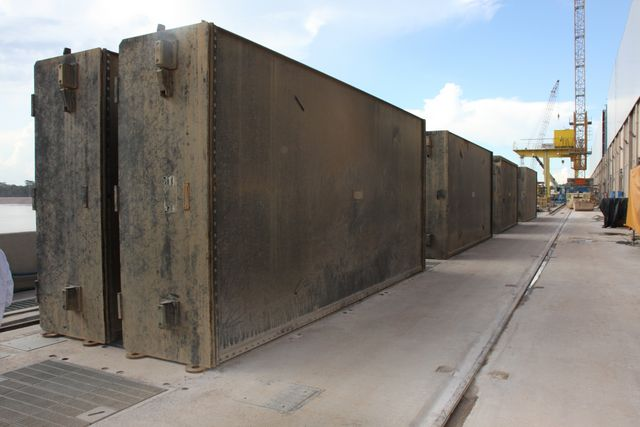
\includegraphics[width=0.9\columnwidth]{figs/nomenclatura/1.jpg}
    \caption{Stoplogs.}
    \label{nomenclatura_1}
\end{figure}

\begin{figure}[H]
    \centering
    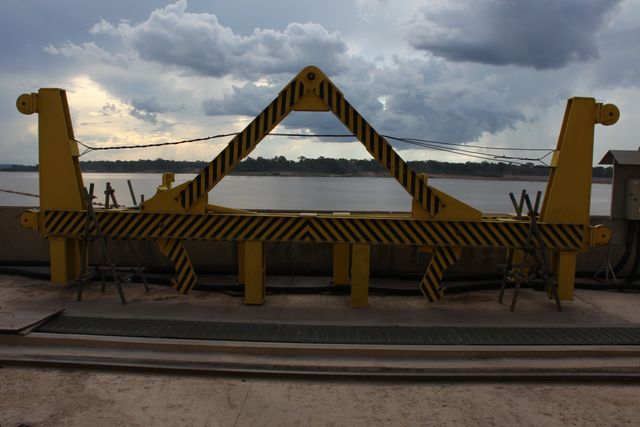
\includegraphics[width=0.9\columnwidth]{figs/nomenclatura/2.jpg}
    \caption{\emph{Lifting Beam}.}
    \label{nomenclatura_2}
\end{figure}


\begin{figure}[H]
    \centering
    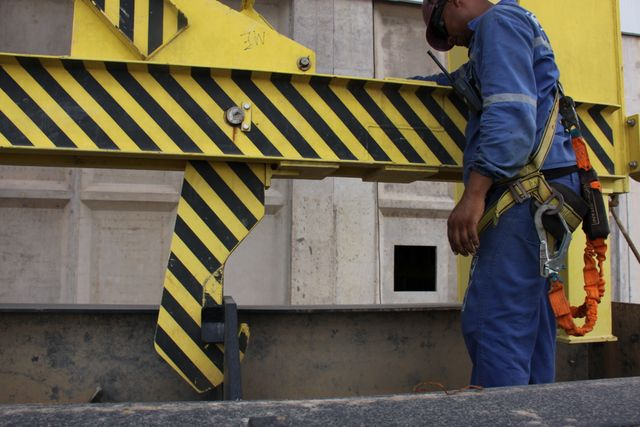
\includegraphics[width=0.9\columnwidth]{figs/nomenclatura/4.jpg}
    \caption{\emph{Garra pescadora}.}
    \label{nomenclatura_4}
\end{figure}

\begin{figure}[H]
    \centering
    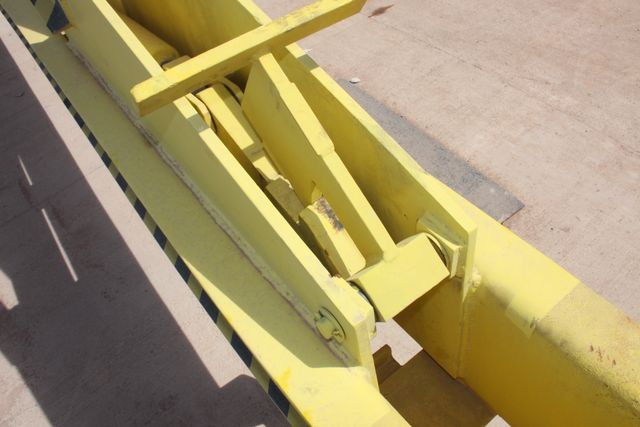
\includegraphics[width=0.9\columnwidth]{figs/nomenclatura/5.jpg}
    \caption{\emph{Chave de operação}.}
    \label{nomenclatura_5}
\end{figure}

\begin{figure}[H]
    \centering
    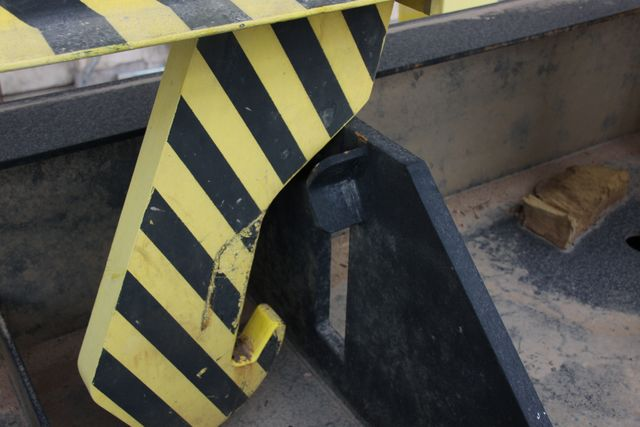
\includegraphics[width=0.9\columnwidth]{figs/nomenclatura/nomenclatura_6.jpg}
    \caption{\emph{Olhal}.}
    \label{nomenclatura_6}
\end{figure}

\begin{figure}[H]
    \centering
    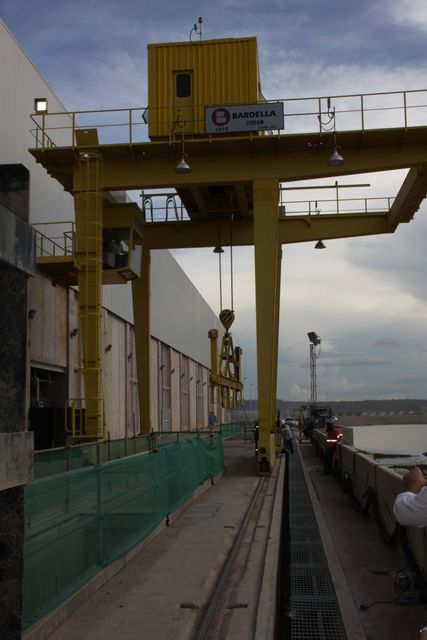
\includegraphics[width=0.9\columnwidth]{figs/nomenclatura/3.jpg}
    \caption{\emph{Guindaste}.}
    \label{nomenclatura_3}
\end{figure}

%%%******************************************************************************
%%
%% introduction.tex
%%
%%******************************************************************************
%%
%% Title......: Introduction
%%
%% Author.....: GSCAR-DFKI
%%
%% Started....: Nov 2013
%%
%% Emails.....: renan028@gmail.com
%%
%% Address....: Universidade Federal do Rio de Janeiro
%%              Caixa Postal 68.504, CEP: 21.945-970
%%              Rio de Janeiro, RJ - Brasil.
%%
%%******************************************************************************


%%******************************************************************************
%% SECTION - Introdu��o
%%******************************************************************************

\section{Introdu��o}
O objetivo deste relat�rio � apresentar o conceito do projeto ROSA. Este documento apresentar� os modos de opera��o do sistema atual e suas falhas, descrever� o sistema proposto, as poss�veis solu��es e a metodologia de pesquisa para o desenvolvimento de solu��es. Por �ltimo, este relat�rio mostrar� um fluxograma completo da opera��o com o novo sistema.

Este relat�rio se organiza nas seguintes se��es:
    \begin{itemize}
        \item Descri��o do problema: descri��o do problema e os modos de opera��o do processo atual.
        \item Sistema proposto: especifica��o do sistema proposto, como sensores e atuadores que ser�o utilizados para a conclus�o dos objetivos do projeto.
        \item Metodologia: descri��o do m�todo de pesquisa e desenvolvimento de solu��es do grupo.
        \item Pesquisa bibliogr�fica: levantamento das tecnologias utilizadas no sistema proposto e as tecnologias estudadas durante a fase de desenvolvimento do sistema.
        \item Fluxograma da solu��o: diagrama l�gico com as etapas do processo, falhas e solu��es.
        \item Refer�ncias.
    \end{itemize}

Faz-se necess�ria a introdu��o da terminologia que ser� utlizada durante este relat�rio:
\begin{itemize}
\item \emph{\emph{Stoplog}}: bloco de a�o com vinte metros de comprimento, tr�s metros de altura e tr�s metros de largura (20x3x3 m). O fluxo de �gua do rio � controlado pelo empilhamento de \emph{Stoplog}s. (FIGURA)
\item \emph{Lifting Beam}: � a estrutura mec�nica respons�vel pelo deslocamento de \emph{Stoplog}s, composta por: duas garras n�o atuadas, duas chaves de opera��o, vigas e mecanismo. Um guindaste atua neste mecanismo. (FIGURA)
\item \emph{Garra pescadora}: garra localizada no \emph{Lifting Beam} que se prende ao \emph{Stoplog}. O mecanismo � composto por duas garras. (FIGURA)
\item \emph{Chave de opera��o}: localizada na viga principal, pr�xima � garra pescadora, seleciona o modo de opera��o.  Atuada manualmente.
\end{itemize}

%% %******************************************************************************
% % % modos.tex %
% %******************************************************************************
% % % Title......: Modos de Operação % % Author.....: GSCAR-DFKI % %
% Started....: Nov 2013 % % Emails.....: renan028@gmail.com, elael@poli.ufrj.br
% & alcantara@poli.ufrj.br % % Address....:
% Universidade Federal do Rio de Janeiro %              Caixa Postal 68.504,
% CEP: 21.945-970 %              Rio de Janeiro, RJ - Brasil.
% %
% %******************************************************************************


% %******************************************************************************
% % SECTION - Modos de Operação
% %******************************************************************************
\chapter{Descrição do problema}
Esta seção descreve o problema que será atacado a partir dos modos de operação
executados durante o processo de vedação do rio.

\section{Viagem de Reconhecimento}
A viagem à Usina Jirau aconteceu entre os dias 10 e 13 de Novembro de 2013. A
equipe era formada por Patrick Paranhos, Ramon Romankeviciuz, Alessandro
Jacoud e Julia Campana. A viagem teve um caráter inicial, o objetivo foi realizar a
reunião de abertura, passando por  uma análise inicial do problema, assim como a
análise de uma operação de \emph{Stoplog}. Complementarmente, a visita proporcionou ao
grupo a oportunidade de conhecer pessoalmente os responsáveis pelo projeto na
ESBR.
Na reunião de abertura, foram esclarecidas questões de ordem técnica e também
questões ligadas aos procedimentos da ESBR em Projetos de Pesquisa e Desenvolvimento -
(P$\&$D).  Por parte da ESBR estavam presentes Breno Mollinati, Ramon Campos e
Gizele Ferreira. Após a reunião de abertura, a equipe foi conduzida a um
pequeno passeio de reconhecimento pela usina a fim de conhecer melhor as
instalações e as atividades lá realizadas, como pode ser observado nas
figs.
(\ref{fig:jirau1},\ref{fig:jirau2},\ref{fig:jirau3},\ref{fig:jirau6}).

 \begin{figure}[ht!]
    \centering 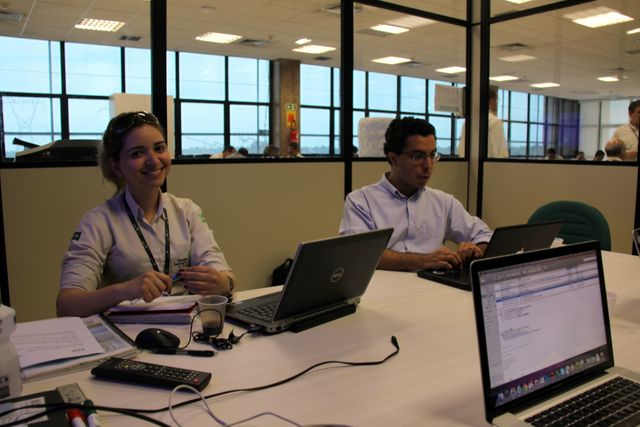
\includegraphics[width=0.6\columnwidth]{figs/jirau/jirau_01}
    \caption{Reunião de abertura.}
    \label{fig:jirau1}
\end{figure}

 \begin{figure}[ht!]
    \centering 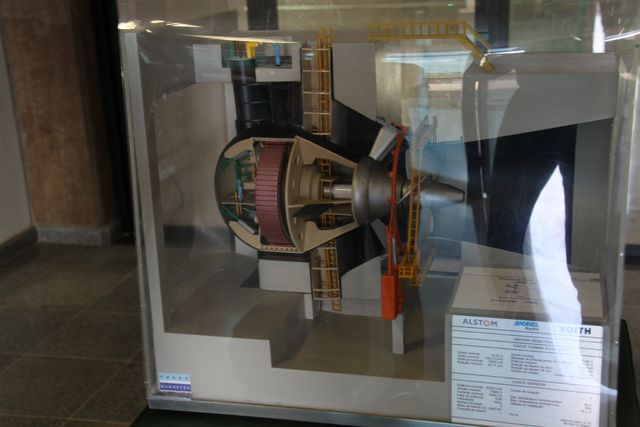
\includegraphics[width=0.6\columnwidth]{figs/jirau/jirau_02}
    \caption{Modelo de turbina da Usina Jirau, observado durante o passeio da
    Usina.}
    \label{fig:jirau2}
\end{figure}

\begin{figure}[ht!]
    \centering 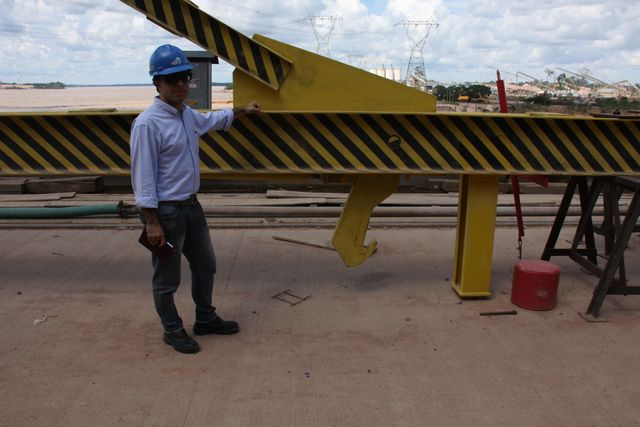
\includegraphics[width=0.6\columnwidth]{figs/jirau/jirau_03}
    \caption{Alessandro Jacoud, observando o lifting beam da garra pescadora.}
    \label{fig:jirau3}
\end{figure}


\begin{figure}[ht!]
    \centering 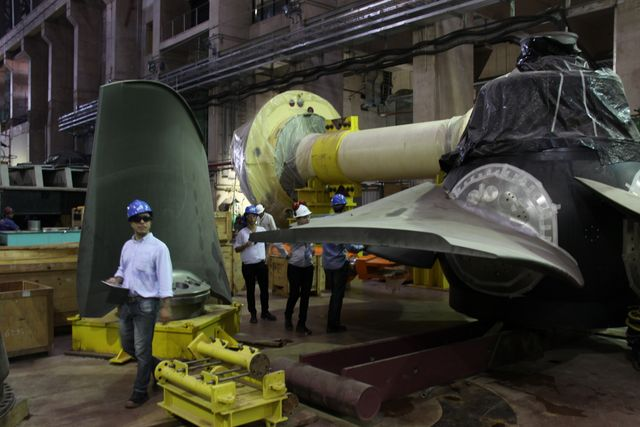
\includegraphics[width=0.6\columnwidth]{figs/jirau/jirau_06}
    \caption{Equipe conhecendo a montagem de turbinas.}
    \label{fig:jirau6}
\end{figure}



\clearpage

Posteriormente à reunião de abertura e ao passeio pela usina, 
o grupo realizou a reunião de análise inicial do problema, onde os problemas
existentes nas operações de inserção e remoção de\emph{Stoplogs} foram
discutidos.
Por fim, foi feita a visita de campo para o acompanhamento da operação de
Stoplog, visando uma melhor compreensão por parte dos pesquisadores da
metodologia e equipamento envolvido nas operações de\emph{Stoplogs}. As Figuras
(\ref{fig:jirau9},\ref{fig:jirau11},\ref{fig:jirau13},\ref{fig:jirau14},\ref{fig:jirau15},\ref{fig:jirau16},\ref{fig:jirau17},\ref{fig:jirau18},\ref{fig:jirau19},\ref{fig:jirau20},\ref{fig:jirau21},\ref{fig:jirau22}).
ilustram o acompanhamento à operação de inserção e remoção de um \emph{Stoplog}.

\begin{figure}[h!]
    \centering 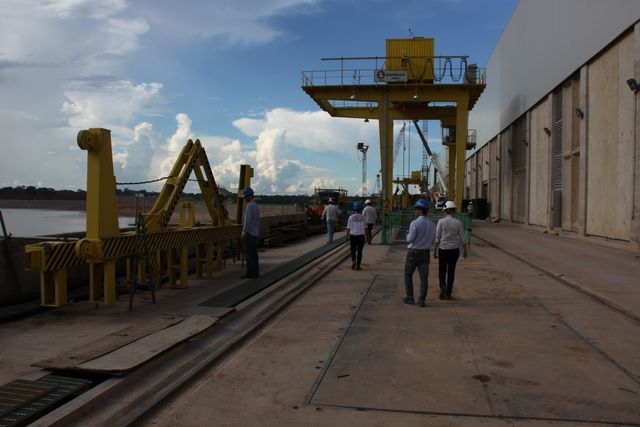
\includegraphics[width=0.6\columnwidth]{figs/jirau/jirau_09}
    \caption{Visita de Campo.}
    \label{fig:jirau9}
\end{figure}

\begin{figure}[h!]
    \centering 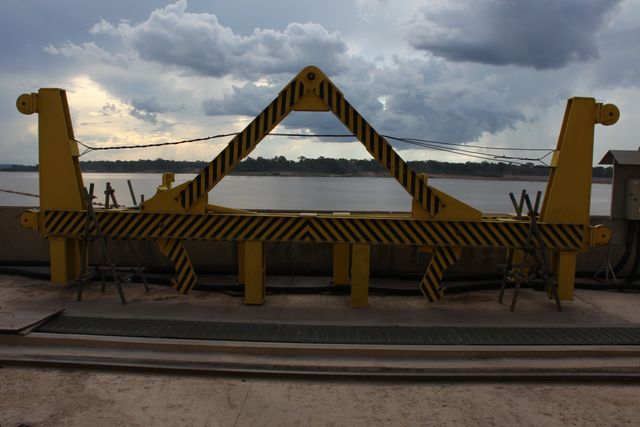
\includegraphics[width=0.6\columnwidth]{figs/jirau/jirau_11}
    \caption{Vista frontal do \emph{Lift beam}.}
    \label{fig:jirau11}
\end{figure}

\begin{figure}[h!]
    \centering 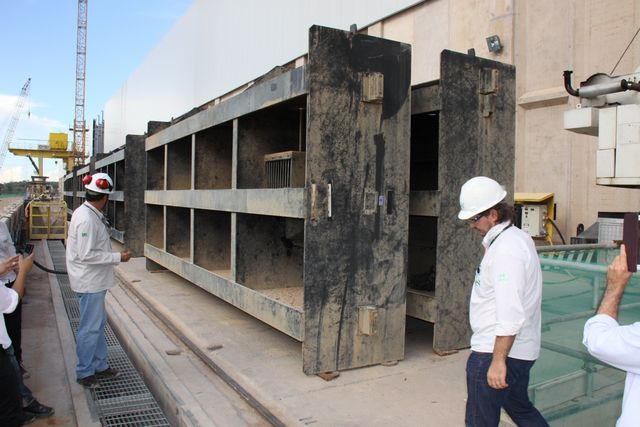
\includegraphics[width=0.6\columnwidth]{figs/jirau/jirau_13}
    \caption{Peça de \emph{Stoplog}.}
    \label{fig:jirau13}
\end{figure}

\begin{figure}[h!]
    \centering 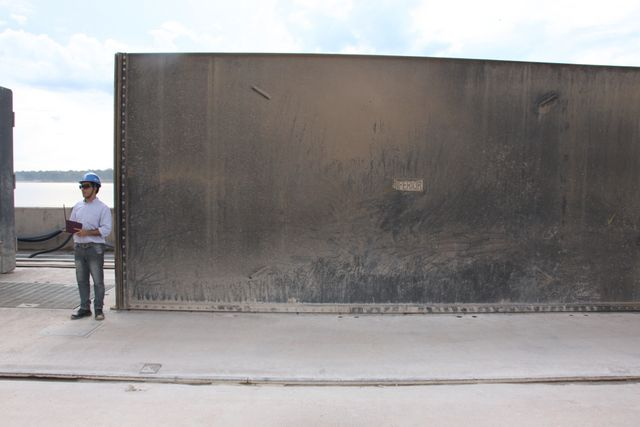
\includegraphics[width=0.6\columnwidth]{figs/jirau/jirau_14}
    \caption{Peça de \emph{Stoplog}.}
    \label{fig:jirau14}
\end{figure}

\begin{figure}[h!]
    \centering 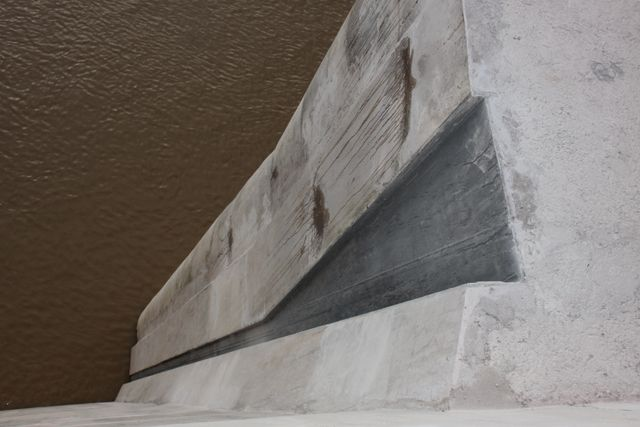
\includegraphics[width=0.6\columnwidth]{figs/jirau/jirau_15}
    \caption{Trilho para as peças de \emph{Stoplog}.}
    \label{fig:jirau15}
\end{figure}

\begin{figure}[h!]
    \centering 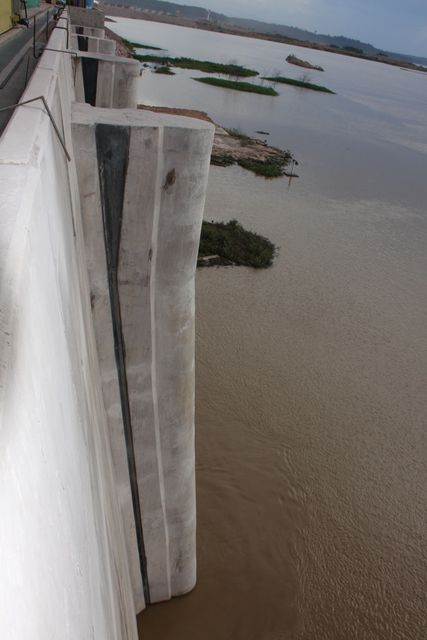
\includegraphics[scale=0.6]{figs/jirau/jirau_16}
    \caption{Trilho para as peças de \emph{Stoplog}.}
    \label{fig:jirau16}
\end{figure}

\begin{figure}[h!]
    \centering 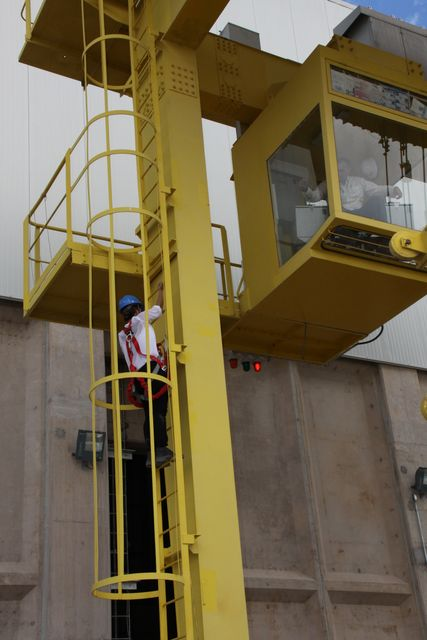
\includegraphics[scale=0.6]{figs/jirau/jirau_17}
    \caption{Parte da análise inclui a observação da operação de \emph{Stoplog} dentro da cabine do operador.}
    \label{fig:jirau17}
\end{figure}

\begin{figure}[h!]
    \centering 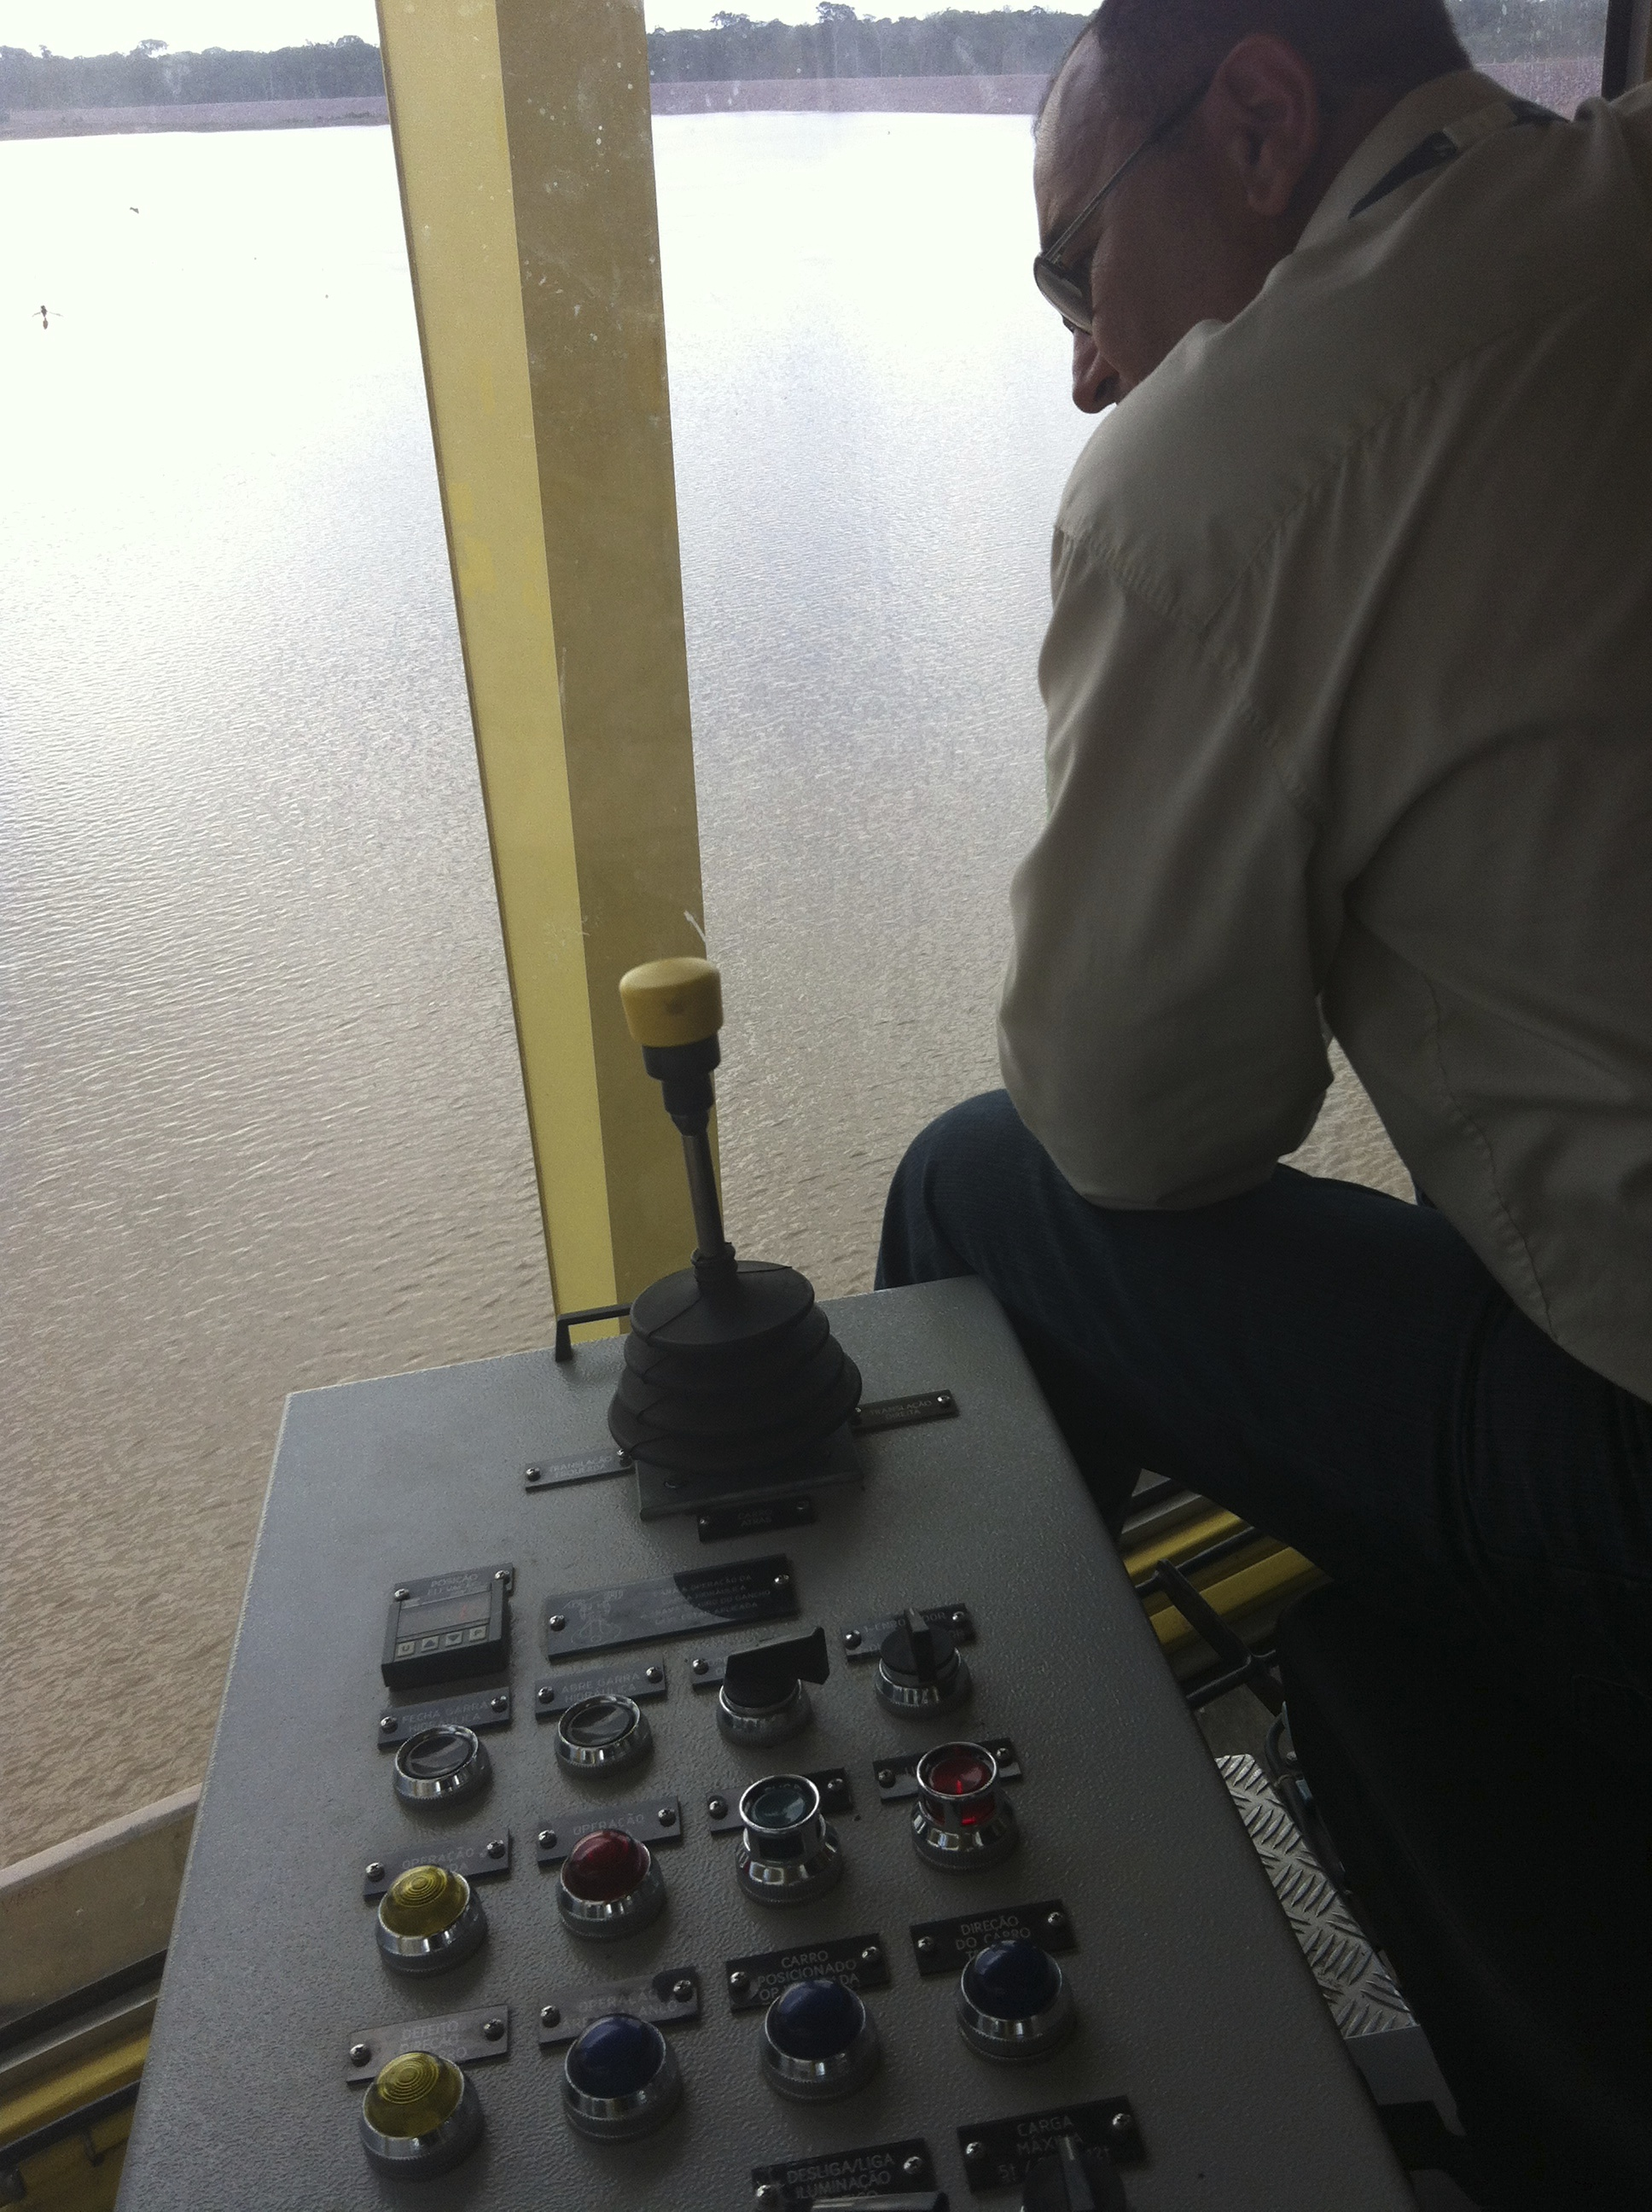
\includegraphics[width=0.6\columnwidth]{figs/jirau/jirau_18}
    \caption{Operador de Portigo Rolante.}
    \label{fig:jirau18}
\end{figure}

\begin{figure}[h!]
    \centering 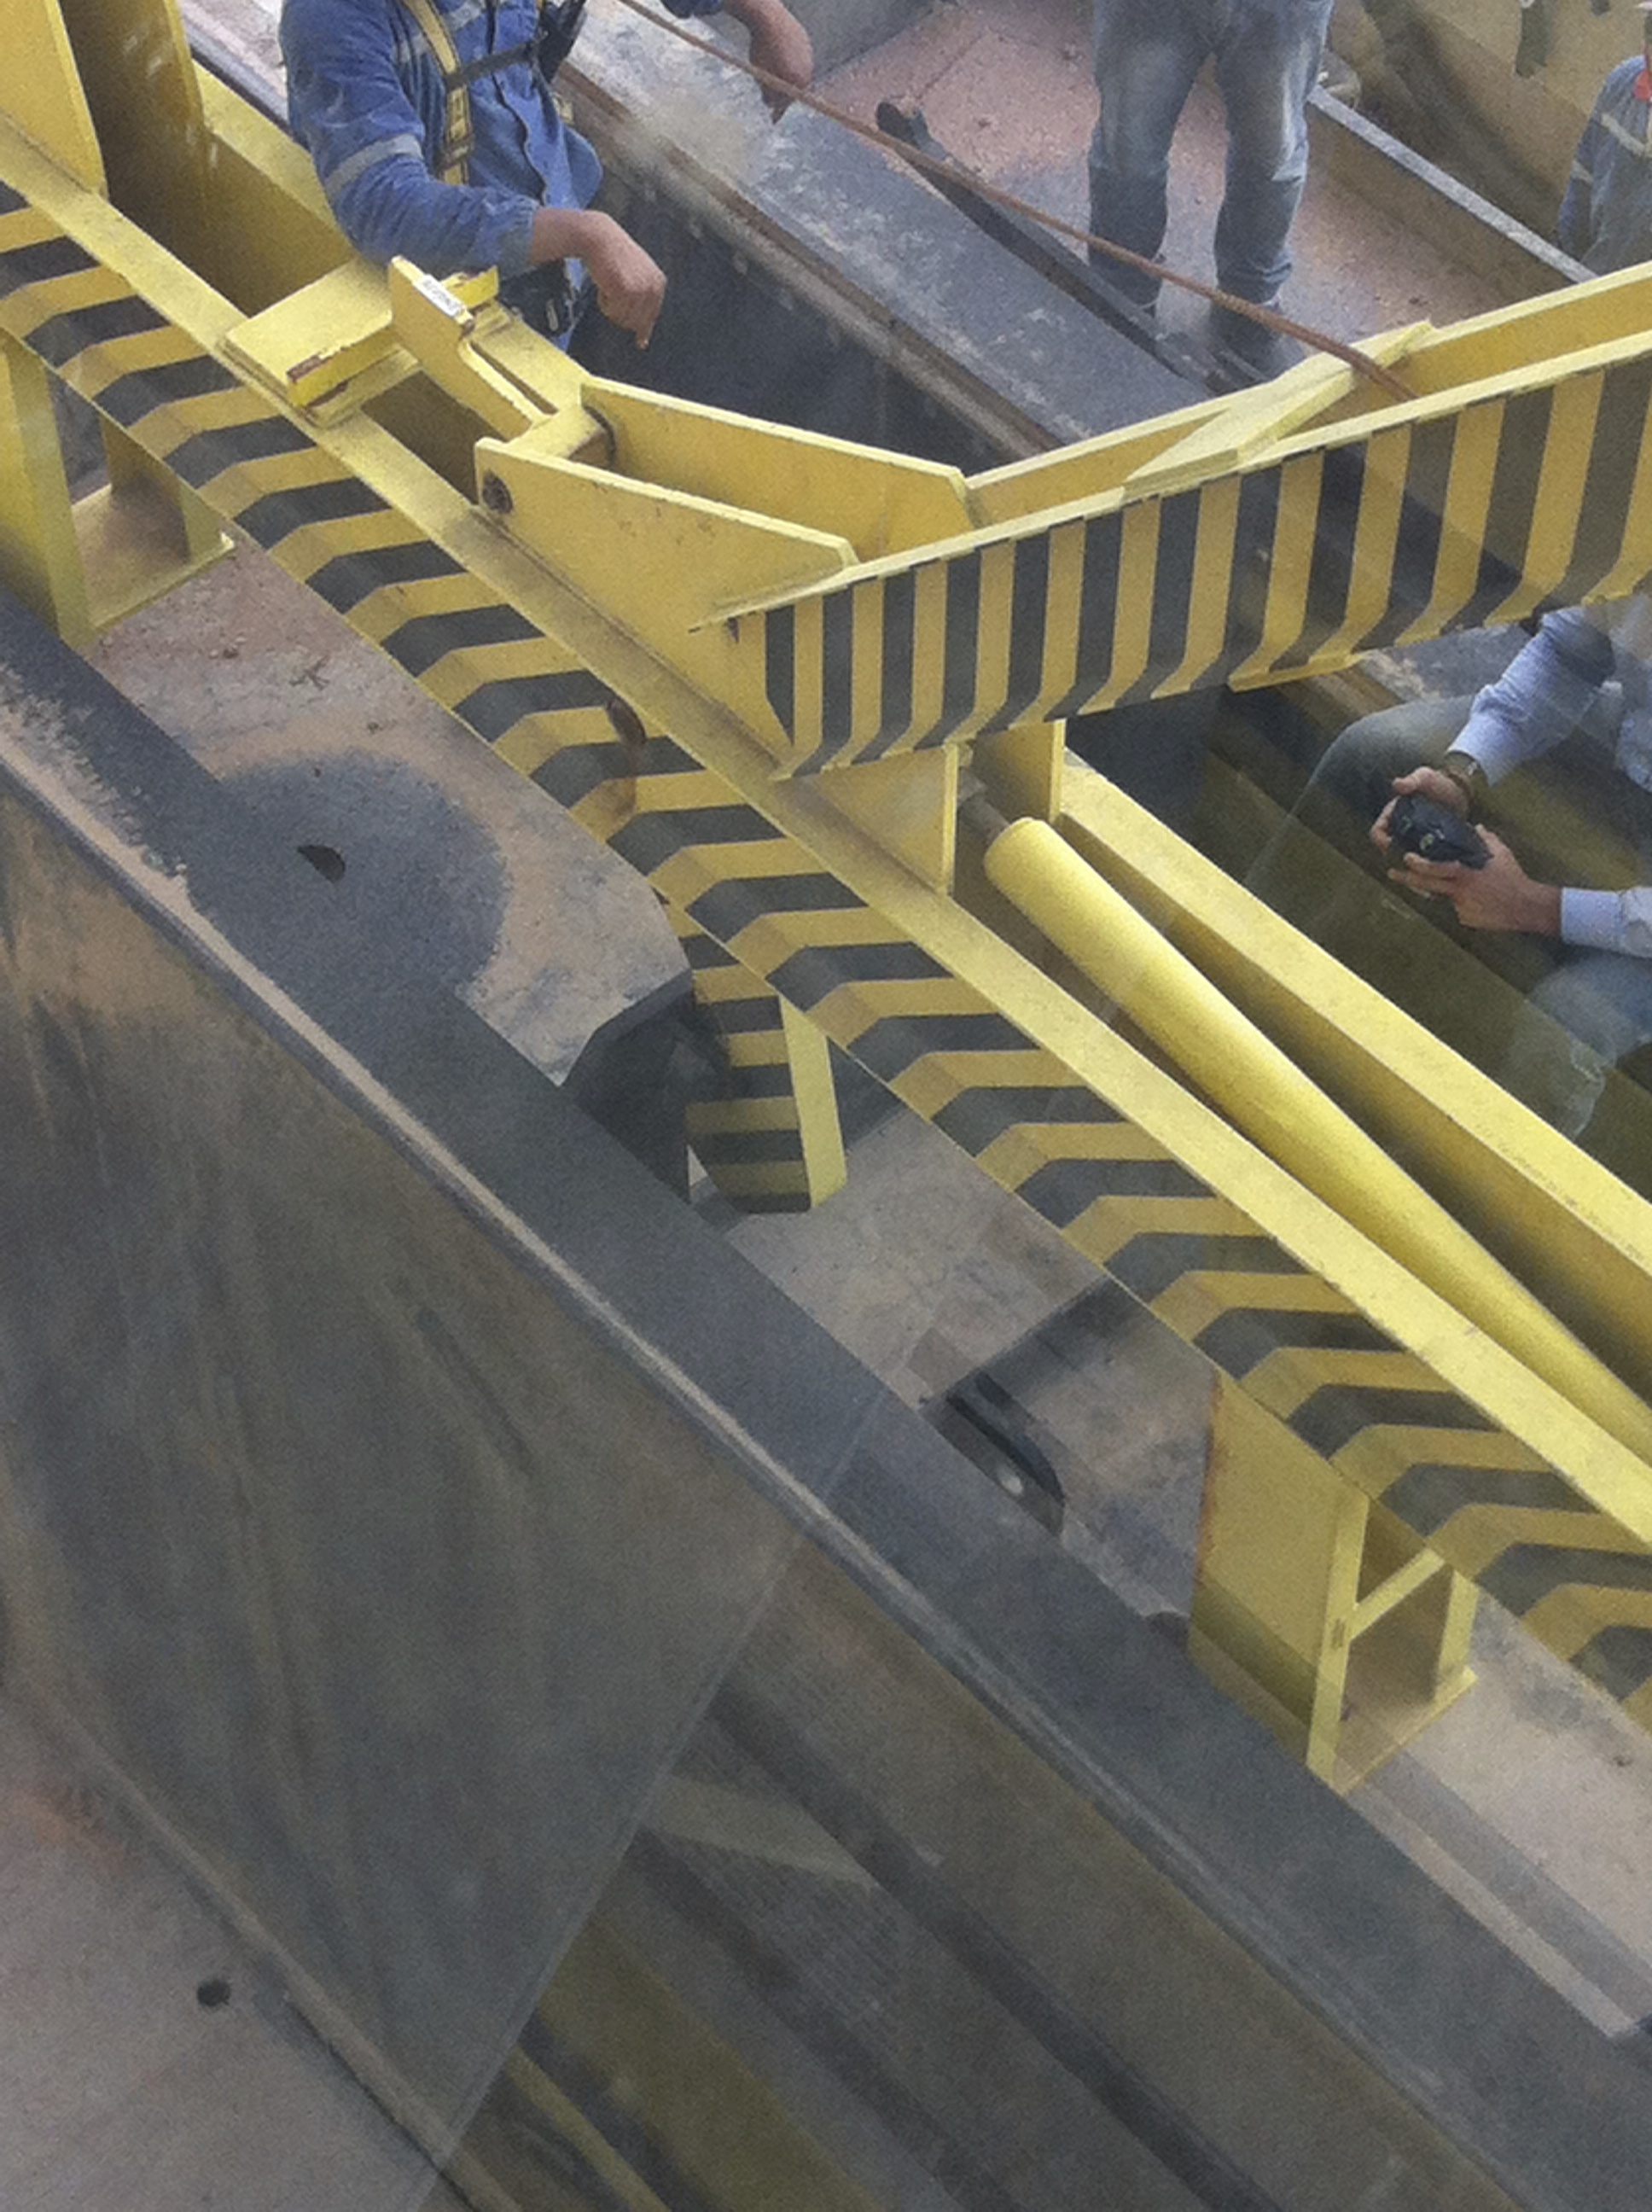
\includegraphics[width=0.5\columnwidth]{figs/jirau/jirau_19}
    \caption{Ponto de vista do \emph{Stoplog} a partir da cabine do operador do pórtigo rolante.}
    \label{fig:jirau19}
\end{figure}

\begin{figure}[h!]
    \centering 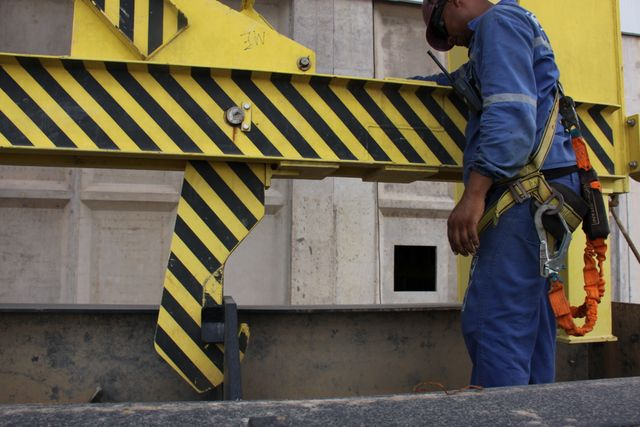
\includegraphics[width=0.6\columnwidth]{figs/jirau/jirau_20}
    \caption{A análise de operação, processo de engate de das garras pescadoras vista 1.}
    \label{fig:jirau20}
\end{figure}

\begin{figure}[h!]
    \centering 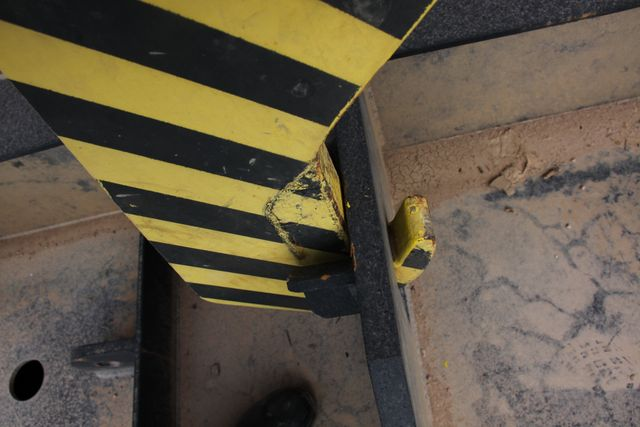
\includegraphics[width=0.6\columnwidth]{figs/jirau/jirau_21}
    \caption{A análise de operação, processo de engate de das garras pescadoras vista 2.}
    \label{fig:jirau21}
\end{figure}

\begin{figure}[h!]
    \centering 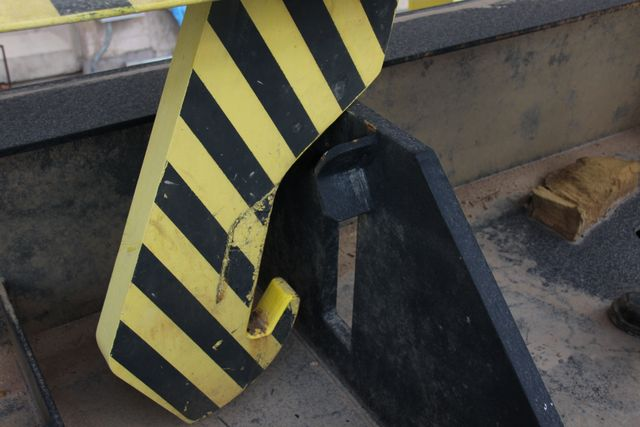
\includegraphics[width=0.6\columnwidth]{figs/jirau/jirau_22}
    \caption{A análise de operação, processo de desengate de das garras pescadoras.}
    \label{fig:jirau22}
\end{figure}



\clearpage

\chapter{Operações Padrão}
Este capítulo é subdividida em dois modos de operação padrão: inserção e remoção
de \emph{Stoplogs}. Cada modo de operação padrão possui três modos de operações
excepcionais, realizados em caso de falhas discutidas durante esta seção.

% %******************************************************************************
% % SUBSECTION - Subsection
% %******************************************************************************


\section{Operação padrão de inserção}
A operação padrão de inserção consiste: inserção de \emph{Stoplogs} no Rio
Madeira para o controle de seu fluxo de água, a fim de realizar a manutenção de
turbinas de um sistema de geração de energia elétrica. Esta operação assume as
seguintes \textbf{hipóteses}:
\begin{enumerate}
\item O trilho está livre de obstáculos e sedimentos que poderiam impedir a execução da tarefa.
\label{hip:ins:1}
\item O conjunto \emph{ Lifting Beam}/\emph{stoplog } não sofre inclinações e
desnivelamento em relação ao trilho, portanto o \emph{stoplog} desliza pelo
trilho sem travamento. \label{hip:ins:2}
\item O desencaixe do conjunto \emph{Lifting Beam}/\emph{stoplog} é realizado
com sucesso. \label{hip:ins:3}
\item O primeiro \emph{stoplog} a ser inserido é posicionado corretamente e veda a base do trilho.
\label{hip:ins:4}
\end{enumerate}

A operação de inserção de \emph{Stoplogs} é composta pelas seguintes
\textbf{etapas}:
\begin{enumerate}
\item Auxiliar de operação manualmente modifica o estado da \emph{chave de operação} para \textbf{Encaixe}.
\item Operador controla o guindaste, o qual desloca o conjunto \emph{Lifting Beam} e \emph{Garras Pescadoras}, 
até a posição do \emph{Stoplog}, que se encontra em terra, e realiza o encaixe. O encaixe bem sucedido é caracterizado 
pelo acoplamento correto das duas garras pescadoras com o \emph{Stoplog}.
\item Auxiliar de operação manualmente modifica o estado da chave de operação para \textbf{Desencaixe}.
\item Operador controla o guindaste, o qual desloca o \emph{Lifting Beam} junto com o \emph{Stoplog}, até os trilhos localizados na barragem, onde os \emph{Stoplogs} deverão ser empilhados.
\item Operador desce o conjunto \emph{Lifting Beam} e \emph{Stoplog} guiado pelo trilho.
\item O desencaixa do conjunto \emph{Lifting Beam}/\emph{Stoplog} é realizado quando o conjunto é impedido de continuar seu curso. Isso ocorre pelo contato do \emph{Stoplog} com o fim da guia ou pelo contato com outro \emph{Stoplog} que já tinha sido posicionado (empilhamento). O desencaixe ocorre, pois, no contato, há perda de tensão no cabo de sustentação do \emph{Lifting Beam} e de forma mecanicamente passiva a garra abre.
\item O procedimento é repetido até que haja \emph{Stoplogs} suficientes para impedir o fluxo de água.
\end{enumerate}

Durante todo o procedimento de inserção, o operador pode monitorar o nível de
tensão no cabo exercido ao \emph{Lifting Beam} pelo motor elétrico. Um sensor de
força strain gauge é responsável por essa informação, porém há complicações em sua
calibração. Dessa forma, o operador infere o nível de tensão aplicado de acordo
com o ruído sonoro gerado pelo motor.

\section{Operação excepcional de inserção 1 - Travamento durante inserção}

Durante a descida do conjunto  \emph{Lifting Beam}/\emph{Stoplog} pelo operador (etapa 5 da operação padrão de inserção), se assumirmos que o trilho não está livre de obstáculos, detritos ou que possui alguma deformação da estrutura do trilho, existe a possibilidade do \emph{stoplog} começar a se inclinar (falsas as
hipóteses 1 e 2), o que pode gerar o travamento da operação.

Ao notar o travamento, o operador continuamente ergue e desce o
conjunto \emph{Lifting Beam}/\emph{Stoplog} em um 
processo de tentativa e erro, até a tarefa ser realizada com
sucesso.

Caso o grau de inclinação do \emph{Stoplog} seja acentuado, o mesmo pode travar completamente no trilho. O risco 
de tal acontecimento é que o desencaixe entre a \emph{Garras Pescadoras} e o \emph{Stoplog}, durante o processo de inserção, 
é  mecânicamente passivo. Logo, existe a possibilidade de haver uma perda de
tração no cabo dado o travamento, o que acarretará em desengate parcial ou total
prematuro do \emph{Stoplog}.

Em caso de desencaixe parcial (apenas uma das
garras) será necessário o envio de um equipe de mergulhadores para corrigir o
problema. Essa operação é lenta e de alto risco de vida, durante a qual o
sistema hidráulico está inoperante.

Em caso de desengate total prematuro, o \emph{Stoplog} cai até o solo sem
controle, podendo resultar em danos a estrutura. Neste caso, é necessário um
processesso de inspeção por mergulhadores para determinar a extensão do dano causado e para recuperação do \emph{Stoplog}.




\section{Operação excepcional de inserção 2 - Falha do desencaixe da garra pescadora}
\label{op:ins:2}

Existe a possibilidade de ao final da operação de inserção não haver o correto desengate do \emph{Stoplog}. 
Esta falha pode ser parcial, apenas uma das \emph{garras pescadoras} se mantém acoplada, ou total, ambas as 
\emph{garras pescadoras} se mantém acopladas. O operador só pode inferir a
ocorrência de um desengate mal sucedido pela tração do cabo do guindaste ao tentar levantar o \emph{Lifiting Beam}.

Ao notar a falha no desengate, o operador continuamente ergue e desce o
conjunto \emph{Lifting Beam}/\emph{Stoplog} em um 
processo de tentativa e erro, até a tarefa ser realizada com sucesso. Entretanto, se o desengate for parcial existe o risco do \emph{Stoplog} inclinar no trilho, resultando em seu subsequente travamento. Atualmente, o único modo de solucionar e determinar a natureza do problem é através do envio de mergulhadores. 

\section{Operação excepcional de inserção 3 - Não vedamento devido ao acumulo de detritos na base do trilho}


Uma violação da \textbf{hipótese} \textbf{\ref{hip:ins:1}}, ou seja, existência
de sedimentos ou obstáculos, nesse caso no fundo do rio, pode acarretar em um mau posicionamento do
\emph{stoplog} resultando em uma má vedação do circuito hidráulico (falha da \textbf{hipótese} \textbf{\ref{hip:ins:4}}).  A falha na vedação acarreta que não seja possivel a drenagem do circuito hidráulico, resultando em atrasos na inspeção planejada e no retorno da geração. 

Atualmente, o único método possível para averiguação da causa da obstrução e solucionamento do problema é através do envio de mergulhadores.  


%_________


\section{Operação padrão - Remoção}
A operação padrão de remoção consiste em, basicamente, a operação inversa à da inserção de \emph{Stoplogs}. Esta operação assume as seguintes \textbf{hipóteses}:

\begin{enumerate}
\item Encaixe bem sucedido entre o conjunto \emph{Lifting Beam}/\emph{stoplog}
realizado dentro d'água.
\item Não há acúmulo de sedimentos entre \emph{stoplogs} e entre \emph{stoplog} e base do trilho. Dessa forma, não há diferença extra de pressão hidrostática a ser vencida pelo \emph{Lifting Beam}.
\label{hip:rem:2}
\item O conjunto \emph{Lifting Beam}/\emph{stoplog} se movimenta livremente pelo trilho, sem obstáculos e sedimentos.
\item O conjunto \emph{Lifting Beam}/\emph{stoplog} é removido do trilho e depositado em solo sem sofrer inclinações.  
\item O desencaixe do conjunto \emph{Lifting Beam}/\emph{stoplog} é realizado com sucesso.
\end{enumerate}

A operação de remoção de \emph{Stoplogs} é composta pelas seguintes \textbf{etapas}:
\begin{enumerate}
\item Auxiliar de operação manualmente modifica o estado da \emph{chave de operação} para \textbf{Encaixe}.
\item Operador controla o guindaste, o qual desloca o conjunto \emph{Lifting
Beam} pelo trilho até a posição do \emph{Stoplog}, submerso. O encaixe bem
sucedido é realizado dentro d'água.
\item O conjunto \emph{Lifting Beam}/\emph{Stoplog} é removido da barragem pelo trilho. 
\item Auxiliar de operação manualmente modifica o estado da chave de operação para \textbf{Desencaixe}.
\item \emph{Stoplog} é depositado em solo.
\item O procedimento é repetido até todos os \emph{Stoplogs} serem removidos
\emph{Stoplogs}.
\end{enumerate}

\section{Operação excepcional de remoção 1 - Falha no encaixe}
\label{op:rem:1}
O encaixe no olhal do \emph{Stoplog} é realizado de forma passiva e sem feedback
quando a operação é realizada submersa. É importante observar que o operador não
recebe nenhum tipo de feedback com relação a encaixe e desencaixe da garra
pescadora. Como a operação é realizada debaixo d'aguá, sem visibilidade, o
processo de encaixe no \emph{Stoplogs} se torna uma longa série de tentativas e
erros, na qual o \emph{Lifting Beam} é suspenso e submerso inúmeras vezes.

Um encaixe mal sucedido durante a etapa 1 (a hipótese 1 não satisfeita) pode ser
decorrente de uma tentativa de encaixe com o \emph{Lifiting Beam} inclinado ou
por detritos presentes no olhal do \emph{Stoplog} ou em sua superfície. Um
encaixe mal sucedido pode acarretar em um desencaixe durante o percurso ou um
encaixe parcial, ocasionando a queda ou travamento do \emph{Stoplog}
(necessitando a realização da \textbf{Operação excepcional de remoção 2}).

Caso não ocorra nenhum encaixe, é realizada múltiplas tentativas até um encaixe
completo. Entretanto, se não houver sucesso, mergulhadores são enviados para a
inspeção do olhal e da superfície do \emph{Stoplog} a procura de detritos
obstruindo o encaixe.

Em caso de engate parcial (apenas uma das garras), auxiliares mergulhadores
são enviados para alterar a posição da \emph{Chave de Operação}, para a
realização do desencaixe das \emph{Garras Pescadoras}. Quando o engate
parcial não é percebido em tempo hábil, devido a ausência de feedback (operação
submersa), existe o risco de inclinação acentuada do \emph{Stoplog} ao ser
levantado por apenas um olhal, podendo resultar em travemento da operação.



\section{Operação excepcional de remoção 2 - Travamento durante remoção}
\label{op:rem:2}

Caso o conjunto \emph{Lifiting Beam/Stoplog} não possa se mover livremente pelo
trilho (\textbf{hipótese} \ref{hip:ins:3} não satisfeita), o conjunto poderá
começar a se inclinar e, assim, ocasionar um possível travamento do sistema. O único feedback
presente nesse tipo de erro é a tração no cabo do guindaste. O operador continuamente ergue e 
desce o conjunto \emph{Lifting Beam}/\emph{Stoplog} em um processo de tentativa e erro, até a tarefa ser realizada com sucesso.
Caso o problema não seja solucionado, é necessário o envio de mergulhadores para averiguação e correção. 

\section{Operação excepcional de remoção 3 - Acúmulo de sedimentos no fundo}
\label{op:rem:3}
Uma vez que a inserção é realizada com sucesso, mantendo então a \textbf{hipótese}
\textbf{\ref{hip:ins:4}}, pode-se ocorrer um posterior acúmulo de sedimentos na
base, ou seja, uma violação da \textbf{hipótese} \textbf{\ref{hip:rem:2}}.

Os sedimentos acumulados no vão inferior (vide figura \ref{fig:op:rem:3_1}) do
\emph{stoplog} em contato com o solo ocasiona um efeito efeito ventosa. Eles
formam uma barreira que forma uma contenção à pressão hidrostática da água (vide
figura \ref{fig:op:rem:3_2})  eliminando a força devido ao princípio de
arquimedes.

As medidas tomadas atualmente consistem apenas em força bruta. Puxa-se o
\emph{stoplog} com um guindaste com força suficiente para vencer a pressão da
coluna d'água, o que comumente acarreta em danos ao próprio \emph{stoplog} e aos
equipamentos envolvidos.

\begin{figure}[h!]
    \centering
    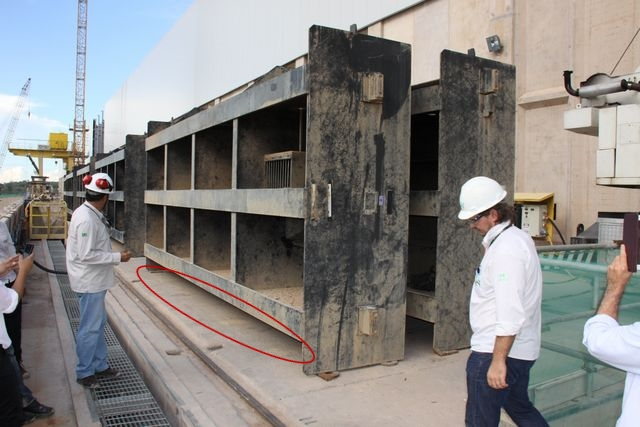
\includegraphics[width=0.6\columnwidth]{figs/modos/op_rem_3/op_rem_3_1.jpg}
    \caption{Local onde ocorre o acúmulo de sedimentos no fundo.}
    \label{fig:op:rem:3_1}
\end{figure}


\begin{figure}[h!]
    \centering
    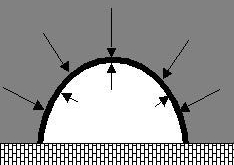
\includegraphics[width=0.6\columnwidth]{figs/modos/op_rem_3/op_rem_3_2.jpg}
    \caption{Pressão interna se torna muito menor que a externa devido ao
    isolamento causado pelos sedimentos.}
    \label{fig:op:rem:3_2}
\end{figure}



%%%******************************************************************************
%%
%% Metodologia.tex
%%
%%******************************************************************************
%%
%% Title......: Introduction
%%
%% Author.....: GSCAR-DFKI
%%
%% Started....: Nov 2013
%%
%% Emails.....: renan028@gmail.com
%%
%% Address....: Universidade Federal do Rio de Janeiro
%%              Caixa Postal 68.504, CEP: 21.945-970
%%              Rio de Janeiro, RJ - Brasil.
%%
%%******************************************************************************


%%******************************************************************************
%% SECTION - Metodologia
%%******************************************************************************

\section{Metodologia}

Com o objetivo de alcan�armos um conceito s�lido foi feita uma pesquisa 




%%%******************************************************************************
%%
%% pesqbib.tex
%%
%%******************************************************************************
%%
%% Title......: Introduction
%%
%% Author.....: GSCAR-DFKI
%%
%% Started....: Nov 2013
%%
%% Emails.....: renan028@gmail.com
%%
%% Address....: Universidade Federal do Rio de Janeiro
%%              Caixa Postal 68.504, CEP: 21.945-970
%%              Rio de Janeiro, RJ - Brasil.
%%
%%******************************************************************************


%%******************************************************************************
%% SECTION - Pesquisa Bibliogr�fica
%%******************************************************************************
% %******************************************************************************
% % % conceito.tex %
% %******************************************************************************
% % % Title......: Projeto Conceitual % % Author.....: GSCAR-DFKI % %
% Started....: Nov 2013 % % Emails.....: renan028@gmail.com % % Address....:
% Universidade Federal do Rio de Janeiro %              Caixa Postal 68.504,
% CEP: 21.945-970 %              Rio de Janeiro, RJ - Brasil.
% %
% %******************************************************************************


% %******************************************************************************
% % SECTION - Sistema proposto
% %******************************************************************************
\section{Projeto Conceitual}
Esta se��o aborda os problemas que ser�o atacados pelo projeto, de acordo com os
modos de opera��o e falhas expostos na se��o Descri��o do Problema.

Conceitualmente, o rob� ROSA ser� constitu�do por um conjunto de sensores e
atuadores a prova d'�gua que ser�o instalados no \emph{Lifting Beam}. Os
sensores e atuadores ser�o conectados a uma eletr�nica embarcada a prova d'�gua,
instalada tamb�m no \emph{Lifting Beam}, que processar� e transmitir� as
informa��es para a superf�cie atrav�s de um umbilical. Na superf�cie, os dados e
controles do sistema poder�o ser visualizados em uma interface gr�fica no
console de comando. Os sensores medir�o dados detalhados sobre o atual status da
opera��o de inser��o/remo��o dos stoplogs permitindo ao operador tomar decis�es
com base nessas informa��es, otimizar a opera��o e evitar poss�veis problemas.
Os atuadores possibilitam intervir na opera��o resolvendo problemas encontrados
sem a necessidade de enviar mergulhadores ao local.

A informa��o de encaixe mal ou bem sucedido entre garra e stoplog � de grande
import�ncia para o operador, durante o processo de remo��o e inser��o. Caso a
opera��o continue sendo executada durante um encaixe mal sucedido, pode haver
danos ao  \emph{Lifting Beam} ao stoplog e ao trilho, al�m de impossibilitar a
finaliza��o da tarefa. H�, portanto, a necessidade de instrumentar a garra
pescadora com sensores que possam fornecer a informa��o de encaixe bem sucedido,
uma eletr�nica embarcada para receber e processar essa informa��o e um sistema
eletr�nico na base que dever� fornecer ao operador o status do processo.
Os principais requisitos de projeto s�o robustez dos dispositivos, capacidade de
submersibilidade (IP69K), resist�ncia a choque, vibra��o, e campos magn�ticos
externos n�o devem afetar as medi��es.

As subse��es que se seguem descrevem o projeto conceitual direcionado a cada
falha de opera��o.

\subsection{Opera��o excepcional de inser��o 1 - Travamento durante inser��o} O
travamento do \emph{stoplog} durante a inser��o pode ser verificado pelo
monitoramento da inclina��o do \emph{Lifting Beam}, pela constante verifica��o
do encaixe a partir do eixo de rota��o das garras e o acompanhamento da
movimenta��o do \emph{Lifting Beam} quando submerso.

Sensores de inclina��o podem fornecer ao operador a informa��o de que o
\emph{stoplog} est� seguindo ou n�o o curso do trilho corretamente.

Mesmo em caso de n�o inclina��o, h� a possibilidade de o \emph{stoplog} ser
assentado de maneira incorreta. O ac�mulo uniforme de sedimentos pode criar uma
camada e impedir o posicionamento correto de \emph{stoplog}. Os sensores de
profundidade possibilitam que o operador monitore a finaliza��o da tarefa.

Sensores de rota��o podem ser acoplados ao eixo de rota��o das garras
pescadoras, monitorando constantemente o encaixe das garras e alertando ao
operador situa��es de inclina��es extremas que estejam desacoplando o conjunto
\emph{Lifting Beam}/\emph{stoplog}.

Vale ressaltar que o projeto conceitual visa o monitoramento da opera��es. O
operador, a partir dos dados recebidos, pode decider em continuar a tarefa ou
reinici�-la.

\subsection{Opera��o excepcional de inser��o 2 - Falha do desencaixe da garra pescadora}
\label{op:sol:ins:1}

As consequ�ncias danosas de um desencaixe mal sucedido entre o \emph{Stoplog} e
as \emph{Garras Pescadoras}, como desencaixe parcial e travamento de
\emph{Stoplogs}, descritas nas subse��es \ref{op:ins:1} e \ref{op:rem:1}, s�o
principalmente devido � falta de feedback na opera��o de inser��o dos
\emph{Stoplogs}.

Devido � geometria do \emph{Lifiting Beam} e das \emph{Garras Pescadoras}, o
desencaixe da \emph{Garra Pescadora} dos \emph{Stoplogs} tem, necessariamente,
um conjunto de posi��es e uma ordem de acontecimento dessas posi��es que a
\emph{Garra Pescadora} deve obedecer. A partir desse fato, � poss�vel monitorar
a opera��o de desencaixe por meio de sensores de rota��o acoplados �s
\emph{Garras Pescadoras}.

Por meio do monitoramento de todas as etapas de movimenta��o das \emph{Garras
Pescadoras} e o alinhamento do \emph{Lifiting Beam}, o operador tem a capacidade
de perceber que a opera��o est� sendo realizada corretamente e caso algum erro
ocorra, pode decidir entre abortar a opera��o e reinici�-la ou, caso seja
necess�rio, aborta-la completamente e tomar a��es corretivas mais dr�sticas,
como o envio de mergulhadores.

A solu��o concebida n�o atua diretamente na movimenta��o das garras e realiza um
desencaixe livre de erros.Entretanto, possibilita um monitoramento de todos os
par�metros fundamentais para uma opera��o correta e eficiente e, assim,  
permite, em tempo real, que ajustes sejam realizados para se finalizar a
opera��o com sucesso ou, se necess�rio,  a opera��o seja abortada para evitar
poss�veis danos ou envio desnecess�rio de mergulhadores.

\subsection{Opera��o excepcional de inser��o 3 - N�o vedamento devido ao acumulo de detritos na base do trilho}

Como forma de evitar o retrabalho, prop�e-se uma inspe��o inicial atrav�s do uso
de um sonar \emph{profiling} que mapear� o fundo do rio e possibilitar� a
identifica��o de detritos presentes. Estes, caso n�o tratados, podem causar
os problemas descritos na subse��o \ref{op:rem:3}.

O mapeamento tamb�m proporciona uma limpeza dos detritos mais eficiente devido
ao conhecimento da localiza��o do que deve ser removido. Limpeza essa feita
por meio de uma bomba submarina capaz de eficientemente remover pequenos
detritos, entretanto para outros de grande porte (e.g. troncos de �rvore
submersos) faz-se necess�rio o uso de um equipamento do tipo garra e guindaste,
j� utilizado atualmente.



\subsection{Opera��o excepcional de remo��o 1 - Falha no encaixe}

O monitoramento da movimenta��o da garra, descrito na subse��o
\ref{op:sol:ins:1}, possibilita de maneira totalmente an�loga um monitoramento
da opera��o de encaixe entre as \emph{Garras Pescadoras} e o \emph{Stoplog}.

Entretanto, se ap�s m�ltiplas tentativas a opera��o de encaixe n�o seja
realizada com sucesso, � poss�vel que haja alguma obstru��o no olhal do
\emph{Stoplog} e/ou em sua superf�cie. Deve-se, ent�o realizar uma opera��o de
inspe��o que possibilite a visualiza��o do problema sem a necessidade do envio
de mergulhadores. Uma vez que a causa do problema e sua localiza��o sejam
identificadas, um sistema de limpeza, controlado remotamente, pode ser enviado.

Para situa��es como a obstru��o do olhal ou pequenos objetos na superf�cie do
\emph{Stoplog} � suficiente a opera��o de limpeza, por�m, em casos extremos,
pode-se usar uma garra ou guindaste extra para auxiliar a elimina��o dos
detritos e, em �ltimo caso, a utiliza��o de mergulhadores.


\subsection{Opera��o excepcional de remo��o 2 - Travamento durante remo��o}
O procedimento � exatamente como no caso da inser��o.

\subsection{Opera��o excepcional de remo��o 3 - Ac�mulo de sedimentos no fundo}
O m�todo para a resolu��o da condi��o de ac�mulo de sedimentos no fundo,
descrita na subse��o \ref{op:rem:3}, n�o faz parte do escopo deste projeto.

%%******************************************************************************
%%
%% pesqbib.tex
%%
%%******************************************************************************
%%
%% Title......: Introduction
%%
%% Author.....: GSCAR-DFKI
%%
%% Started....: Nov 2013
%%
%% Emails.....: renan028@gmail.com
%%
%% Address....: Universidade Federal do Rio de Janeiro
%%              Caixa Postal 68.504, CEP: 21.945-970
%%              Rio de Janeiro, RJ - Brasil.
%%
%%******************************************************************************


%%******************************************************************************
%% SECTION - Pesquisa Bibliogr�fica
%%******************************************************************************
\setcounter{secnumdepth}{5}
\section{Pesquisa Bibliogr�fica e de fornecedores}

\subsection{Sensor de for�a}

 Sensores de for�a podem ser utilizados para detectarem a presen�a da garra pescadora. A an�lise quantitativa e comparativa dessas for�as pode indicar encaixe mal ou bem sucedido durante a opera��o e, portanto, � considerada uma solu��o vi�vel mediante calibra��o. Os diversos tipos de sensores de for�a e suas aplica��es podem ser consultados em \textbf{Guide to the Measurement of Force}, publicado por \textbf{The Institute of Measurement and Control, London}.

 O sensor de for�a � composto por um transdutor, que � submetido � for�a, e uma instrumenta��o associada, respons�vel por alimentar o transdutor e processar a sa�da. O transdutor � um dispositivo que recebe um est�mulo f�sico, como a contra��o el�stica do material devido ao peso, e traduz em outra medida f�sica, como varia��o de voltagem ou corrente el�trica. Esta varia��o obedece uma rela��o conhecida e, dessa forma, � poss�vel determinar quantitativamente a for�a aplicada.

 Existem diversos sensores de for�a dispon�veis no mercado, com sistemas variados de opera��o. As principais caracter�sticas a serem consideradas na escolha de um sensor de for�a s�o: curva de resposta, capacidade m�xima, n�o-linearidade, histerese, sensibilidade e reprodutibilidade.

 O sensor de for�a mais utilizado e que atende aos requisitos do projeto � o strain gauge. A for�a atua em um metal cil�ndrico, que � comprimido e altera a resist�ncia de um strain gauge, acoplado � superf�cie do cilindro (ver figura~\ref{forca_1}).

 \begin{figure}[H]
    \centering
    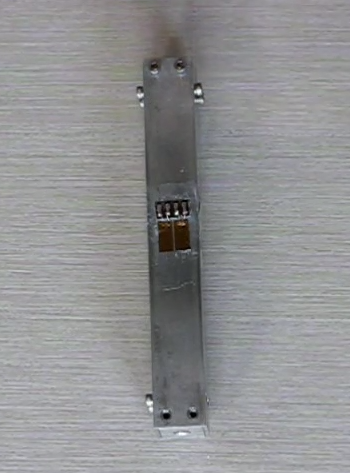
\includegraphics[width=0.4\columnwidth]{figs/forca/1.png}
    \caption{Exemplo de um sensor de for�a: cilindro com strain gauge acoplado.}
    \label{forca_1}
\end{figure}


 A resist�ncia el�trica de um fio varia conforme seu comprimento e sua �rea, portanto, a varia��o de corrente que passa por este fio pode ser utilizada como medida quantitativa e � poss�vel determinar a for�a aplicada por um modelo matem�tico conhecido: $R=\frac{\rho L}{A}$. Outros sensores que poderiam atender �s especifica��es, mas s�o de mais dif�cil comercializa��o, em rela��o aos requisitos de projeto, s�o: sensor de for�a piezoel�trico

 De acordo com \textbf{Guide to the Measurement of Force}, a aplica��o pode ser caracterizada como sistema para medi��es e controle de for�as para opera��es de seguran�a. Pode ainda ser especificada como \textbf{Crane overload/underload protection}, que consiste em monitorar for�as atuando em garras tipo pescadora ou gancho (ver figura~\ref{forca_2}), no qual a medida ser� avaliada em situa��es est�ticas ou de pouco movimento/vibra��o.

  \begin{figure}[H]
    \centering
    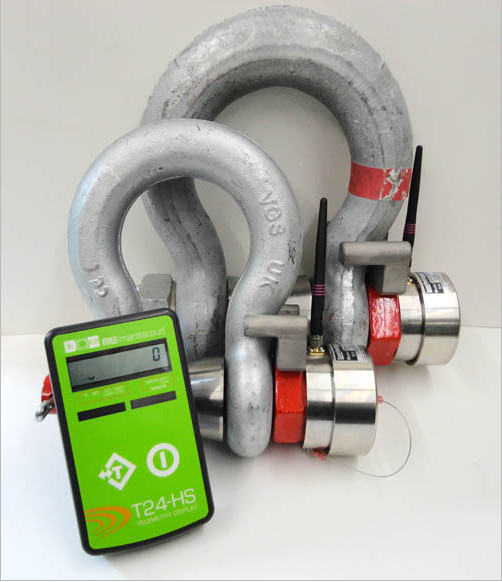
\includegraphics[width=0.4\columnwidth]{figs/forca/2.png}
    \caption{Exemplo de instala��o de sensor de for�a em garra.}
    \label{forca_2}
\end{figure}

 \subsubsection{Conclus�o de an�lise t�cnica}

A solu��o por sensores de for�a � eficiente em aplica��es onde se deseja avaliar frequ�ncia de vibra��o e dura��o da onda de choque, por�m n�o muito na medida quantitativa e comparativa de for�as devido � sensibilidade do strain gauge a campos magn�ticos externos, press�o hidrost�tica e umidade. A varia��o de ac�mulo de sedimentos no stoplog tamb�m dificulta a calibra��o do instrumento.

 \subsubsection{Pesquisa de fornecedores}

Os fornecedores para sensores de for�a do tipo strain gauge avaliados nesta pesquisa s�o: Applied Measurements Limited, Load Cell Central, Transducer Techniques. Os modelos avaliados s�o da s�rie DBEP e CLP de seus respectivos fornecedores.

\subsection{Sensor indutivo de proximidade}

Sensores indutivos de proximidade podem ser utilizados para detectarem a presen�a da garra pescadora. Este sensor de presen�a pode ser do tipo linear, podendo ser realizada an�lise quantitativa, ou simplesmente chaveado, um simples indicador de presen�a. Portanto, pode indicar encaixe mal ou bem sucedido durante a opera��o de remo��o/inser��o de stoplogs. Os sensores indutivos apresentam a mesma forma de opera��o nos diversos produtos dispon�veis no mercado, diferenciando-se principalmente na medida de dist�ncia da aplica��o.

 O sistema para sensoriamento por indu��o magn�tica � composto por uma fonte de alimenta��o e um indutor. Ao alimentar o sensor indutivo, uma corrente alternada � gerada. A corrente el�trica que passa pelo indutor gera um campo magn�tico na face do sensor. Este campo magn�tico induz corrente de Foucault no alvo met�lico, que aumenta conforme o alvo se aproxima do sensor indutivo. O aumento das correntes de Foucault cria um campo magn�tico no alvo, que ir� se opor ao campo produzido pelo sensor indutivo. Essa redu��o do campo magn�tico pode ser medida e, portanto, � poss�vel presenciar o alvo.

 Existem diversos sensores indutivos dispon�veis no mercado que atendem �s especifica��es, apresentam o mesmo modo de opera��o e diferenciam-se principalmente quanto � robustez, instala��o (faceada ou n�o) e interface de sa�da. A resist�ncia a choques, vibra��o, submersibilidade e o tipo de instala��o s�o as caracter�sticas mais importantes para a aplica��o. O sensor deve ser do tipo IP69K e faceado, o que diminui o alcance, mas aumenta a prote��o.

 A pesquisa por sensores indutivos de proximidade para a finalidade desejada resultou em aplica��es equivalentes. A empresa \textbf{HATCH - Energy Innovations} desenvolveu em 2007 um Lifting Beam instrumentado com sensores indutivos (ver figura~\ref{indutivo_1}). Em 2008, a empresa \textbf{Atlas Polar} adotou a mesma solu��o com sensores indutivos.

 \begin{figure}[H]
    \centering
    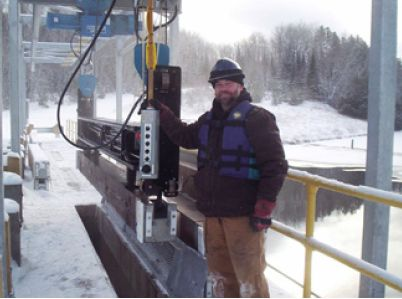
\includegraphics[width=0.5\columnwidth]{figs/indutivo/1.jpg}
    \caption{Lifting Beam desenvolvido pela empresa HATCH}
    \label{indutivo_1}
\end{figure}

 \subsubsection{Conclus�o de an�lise t�cnica}
A solu��o por sensores indutivos � eficiente em aplica��es onde se deseja avaliar a presen�a de stoplog. A grande maioria dos sensores s�o fr�geis a choque e vibra��o, al�m de sens�veis a ru�dos el�tricos e magn�ticos. Por�m, j� h� no mercado produtos IP69K e encapsulados. H�, tamb�m, a possibilidade de falso positivo em caso de sedimentos met�licos, mas � baixa a probabilidade.
Pesquisas em aplica��es semelhantes mostraram que o sensor indutivo � a solu��o adotada para o monitoramento de encaixe entre garra pescadora e stoplog, auxiliado por outros sensores ou sistemas independentes de atuadores.

 \subsubsection{Pesquisa de fornecedores}

Os fornecedores pesquisados para sensores indutivos que atendem aos requisitos de projeto s�o: Contrinex, Pepperl-Fuchs, Positek e Turck. Diversos modelos foram avaliados, juntamente com os t�cnicos das respectivas empresas.
As vantagens apresentadas e a utiliza��o desse tipo de sensoriamento em aplica��es equivalentes foram decisivos para a escolha por esta solu��o em nossa aplica��o. O modelo selecionado, ap�s ampla an�lise entre fornecedores, � o modelo NBB20-L2-E2-V1 de instala��o faceada, chaveado normalmente aberto e dist�ncia de opera��o de 2cm. (FIGURA)

\subsection{Sensor capacitivo de proximidade}
Os sensores capacitivos de proximidade s�o capazes de detectar objetos devido � capacidade destes alvos em serem carregados eletricamente. Analogamente ao sensor indutivo, que detecta varia��es de campo magn�tico devido a alvos met�licos, o sensor capacitivo � sens�vel a varia��es na capacit�ncia (ver figura~\ref{capacitivo_1}).

\begin{figure}[H]
    \centering
    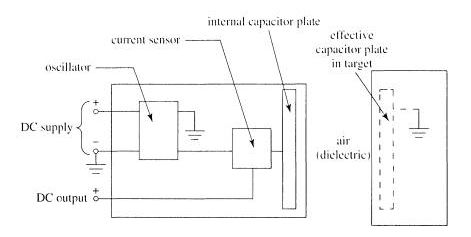
\includegraphics[width=0.8\columnwidth]{figs/capacitivo/1.jpg}
    \caption{Sensor capacitivo}
    \label{capacitivo_1}
\end{figure}

Internamente ao sensor, h� um circuito que utliza a alimenta��o DC para gerar voltagem alternada (oscilador). O circuito interno RC �, ent�o, alimentado e uma corrente alternada passa por esse circuito. O fluxo de corrente alternada depende da capacit�ncia, e esta varia  conforme a dist�ncia e �rea entre as placas do capacitor e o material diel�trico entre as placas: $C = \frac{\epsilon A}{d}$.

Em sensores capacitivos, uma placa do capacitor est� no sensor e a outra � o objeto a ser detectado, que pode ser um material met�lico ou n�o-met�lico. A aproxima��o do alvo modifica a capacit�ncia, resultando em varia��es no campo el�trico e na corrente alternada. Finalmente, as varia��es da corrente podem ser medidas e o alvo � detectado.

As caracter�sticas que devem ser avaliadas em sensores capacitivos s�o as mesmas dos sensores indutivos, como tipo de instala��o, modo de opera��o chaveado ou linear e etc. Por�m, deve-se atentar ao fator de redu��o, que depende do alvo a ser detectado.

 \subsubsection{Conclus�o de an�lise t�cnica}
 Os sensores capacitvos exercem fun��o semelhante ao sensor indutivo e pode ser utilizado para detec��o de presen�a de stoplog. Por�m, a calibra��o se mostra bem mais complexa devido � sensibilidade do sensor e ao fato de n�o estar restrito a detec��o de materiais met�licos. A chance de falsos positivos ser� bem maior em caso de escolha deste sensor em compara��o com o sensor indutivo.
 \subsubsection{Pesquisa de fornecedores}
Os fornecedores pesquisados de sensores capacitivos s�o os mesmos fornecedores de sensores indutivos.

\subsection{Encoder}
O Sistema de Lifting Beam desenvolvido em aplica��o semelhante de remo��o e inser��o de stoplogs pela empresa \textbf{HATCH} utliza atuadores el�tricos independentes em cada garra, o que permite o monitoramento da abertura das garras, sendo poss�vel saber quando h� encaixe mal ou bem sucedido. O sistema em estudo a ser desenvolvido, por�m, � um Lifting Beam mec�nico, onde as garras abrem e fecham passivamente conforme o Lifting Beam � atuado e a chave de opera��o � selecionada em uma determinada posi��o. Por quest�es de restri��o de projeto, n�o � permitido alterar a estrutura mec�nica de forma que as garras sejam atuadas independentemente, mas � permitida a instrumenta��o do Lifting Beam com encoders, sendo poss�vel instal�-los nas vigas das garras, a fim de medir suas posi��es angulares.A movimenta��o angular das garras durante o encaixe � conhecido e sequencial, de forma que uma simples anl�lise comparativa com os dados fornecidos pelos encoders durante a execu��o da tarefa pode indicar se o encaixe foi mal ou bem sucedido.

O encoder �ptico � um dispositivo eletromec�nico que entrega como sa�da um sinal el�trico proporcional � posi��o angular do eixo acoplado. O eixo � acoplado mecanicamente a um disco opaco e marcado em sua superf�cie por segmentos (ver figura~\ref{encoder_1}).

\begin{figure}[H]
    \centering
    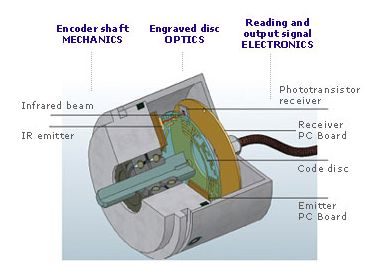
\includegraphics[width=0.5\columnwidth]{figs/encoder/1.jpg}
    \caption{Sistema interno de um encoder.}
    \label{encoder_1}
\end{figure}

Diodos emissores de luz infravermelha alcan�a os receptores atrav�s das fendas do disco. O sinal anal�gico � criado, amplificado, convertido em digital e transmitido ao processador.

Al�m dos requisitos b�sicos do projeto, como submersibilidade e resist�ncia a choque e vibra��o, as principais caracter�sticas a serem avaliadas neste projeto para a escolha de um encoder s�o: modo de opera��o incremental ou absoluto, multi-voltas ou n�o, interface de comunica��o, resolu��o e tens�o de opera��o.

 \subsubsection{Conclus�o de an�lise t�cnica}
A pesquisa mostrou ampla aplica��o de encoders para a aplica��o e � esperado que seja poss�vel identificar encaixe mal ou bem sucedido com sua utiliza��o. A instala��o do encoder na viga da garra pescadora n�o � mecanicamente complexa e n�o resultar� em altera��o permanente da estrutura.

 \subsubsection{Pesquisa de fornecedores}
Os fornecedores para encoders que atendem aos requisitos de projeto pesquisados s�o: Hohner, IFM, Pepperl-Fuchs e Rotary Encoder Solutions.

As vantagens apresentadas e a utiliza��o desse tipo de sensoriamento em aplica��es equivalentes foram decisivos para a escolha por esta solu��o em nossa aplica��o. O modelo selecionado, ap�s ampla an�lise entre fornecedores, � o modelo Encoder RM9000 Absoluto com interface CAN, multi-voltas. (FIGURA)

\subsection{Sensor de campo magn�tico}
O stoplog � um bloco met�lico e esta caracter�stica f�sica pode ser aproveitada em solu��es de circuito magn�tico e el�trico.

Um circuito magn�tico consiste em uma malha fechada que cont�m um fluxo magn�tico atrav�s de condutores. A solu��o estudada � induzir um campo magn�tico em uma garra e utilizar um sensor de campo magn�tico na outra extremidade do Lifting Beam, fazendo com que o pr�prio stoplog seja o condutor. A permeabilidade magn�tica do stoplog � maior do que a permeabilidade da �gua e, dessa forma, o sensor de cmapo magn�tico detectaria varia��es no caso de presen�a de stoplog. (ver figura~\ref{magnetico_1})

\begin{figure}[H]
    \centering
    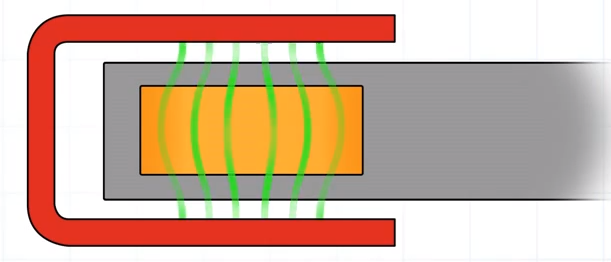
\includegraphics[width=0.5\columnwidth]{figs/magnetico/1.png}
    \caption{Circuito magn�tico.}
    \label{magnetico_1}
\end{figure}


 \subsubsection{Conclus�o de an�lise t�cnica}
Sensores magn�ticos exigem uma �rea de pouca interfer�ncia magn�tica, s�o muito sens�veis e necessitam de calibra��o rigorosa para cada aplica��o. Al�m disso, a dist�ncia entre gerador de campo e sensor � longa devido ao comprimento do stoplog, o que exige ainda maior sensibilidade do sensor e grandes geradores. Esta solu��o n�o foi selecionada.

\subsection{Sensoriamento por campo el�trico}
Outra solu��o semelhante ao circuito magn�tico e que utiliza a vantagem da propriedade f�sica met�lica do stoplog � o circuito el�trico.

O circuito el�trico � formado por uma diferen�a de potencial entre dois terminais em uma malha fechada. Na aplica��o, o stoplog fecha a malha do circuito e ser� equivalente a uma resist�ncia e pode ser realizada tanto a configura��o de divisor de tens�o, como a medi��o da corrente por efeito hall (~\ref{senseletrico_1}).

\begin{figure}[H]
    \centering
    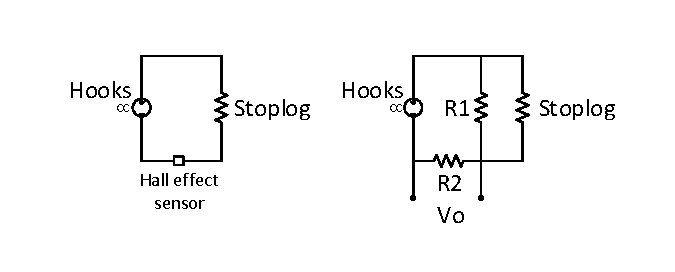
\includegraphics[width=1\columnwidth]{figs/senseletrico/1.pdf}
    \caption{Circuito el�trico}
    \label{senseletrico_1}
\end{figure}


 \subsubsection{Conclus�o de an�lise t�cnica}
 A solu��o apresentada, apesar de eficaz, apenas indica a presen�a de stoplog, n�o o encaixe mal ou bem sucedido. Al�m disso, h� grande possibilidade de sedimentos e ferrugem prejudicarem no sensoriamento do sistema. Esta solu��o n�o foi selecionada.

\subsection{Sonar}
Sonar\footnote{A sigla tem origem como acr�nimo de \textit{sound navigation and ranging}.} � uma t�cnica que utiliza a propaga��o do som na �gua para se comunicar e detectar objetos nesse meio, ela possui duas vertentes uma chamada ativa e outra passiva. A passiva se resume a escutar o meio e n�o ser� investigada, pois n�o possui a funcionalidade para o mapeamento de superf�cies submersas. Os equipamentos que fazem uso de tal tecnologia acabam por herdar seu nome, assim sonares que utilizam a tecnologia ativa s�o chamados de sonares ativos.

O sonar ativo, daqui em diante apenas referido como sonar, emite um ping que � um pulso de onda sonora que ser� refletido pelo meio. Conforme a frente de onda atravessa os objetos submersos ela � refletida e este eco � detectado no retorno pelo sonar, onde ele extrai as informa��es do tempo que a onda levou para retornar e sua intensidade, podendo, a partir do conhecimento de caracter�sticas do meio, como a velocidade de propaga��o do som, estimar a distancia de origem do eco e consequentemente do objeto.

Pela aplica��o os sonares s�o divididos em basicamente duas categorias: \emph{profiling} e \emph{imaging};

O sonar do tipo \emph{imaging} s�o tipicamente utilizados para fazer o mapeamento do fundo do mar, possuindo uma abertura em formato de leque (ver figura~\ref{sonar_1)}), eles podem utilizar um motor de rota��o sobre o eixo perpendicular ao feixe ou podem ser arrastados pela �gua para fazer o escaneamento (ver figura~\ref{sonar_2)}).

\begin{figure}[H]
    \centering
    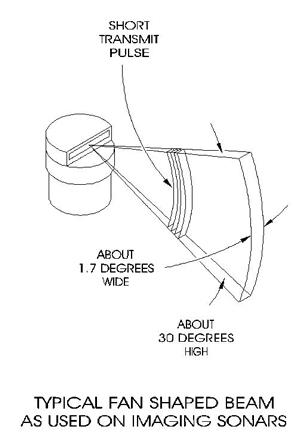
\includegraphics[width=0.5\columnwidth]{figs/sonar/1.jpg}
    \caption{T�pico feixe em formato de leque de sonares tipo \emph{imaging}}
    \label{sonar_1}
\end{figure}

\begin{figure}[H]
    \centering
    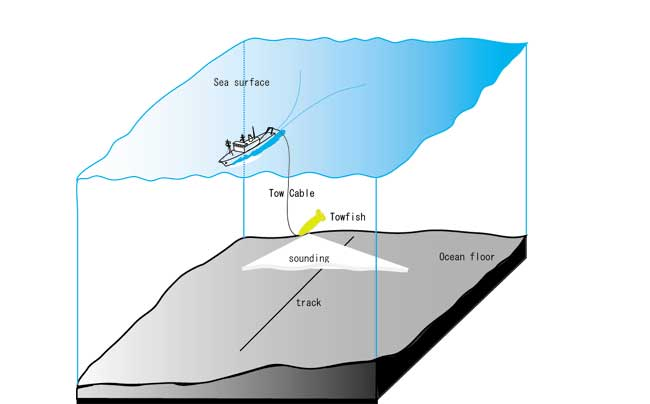
\includegraphics[width=0.5\columnwidth]{figs/sonar/2.jpg}
    \caption{Sonar \emph{imaging} sendo arrastado para mapeamento das profundezas}
    \label{sonar_2}
\end{figure}


A resposta dos sonares tipo \emph{imaging} forma uma imagem colorida exibindo tons diferentes para respostas mais fortes e mais fracas de eco do sonar. Sendo utilizado para obter uma imagem do fundo do mar semelhante as que os radares fazem na superf�cie.

Pela tecnologia empregada os sonares \emph{imaging} possuem dois tipos de configura��o: \emph{multibeam} e \emph{mechanical} (single beam).

A configura��o \emph{single beam} possui um transdutor acoplado a um mecanismo de \emph{pan} para possibilitar a varredura de determinada �rea. Assim, o sonar envia seu \emph{ping} espera o eco de retorno e avan�a para a pr�xima posi��o determinada pelo passo, ou resolu��o angular, do motor que comp�e o mecanismo de \emph{pan}.

Alternativamente, os sonares \emph{multibeam} possuem idealmente um feixe \emph{ping} extremamente amplo, sendo na pr�tica composto por diversos feixes com seus respectivos transdutores sincronizados. Essa configura��o possui diversos receptores espalhados por uma regi�o do sonar, resolvendo qual a posi��o de origem do eco atrav�s de um sistema de multilatera��o. Assim, o \emph{multibeam} sobrepuja a configura��o \emph{single beam} no aspecto de precis�o e tempo de varredura.

De forma diferente, os sonares do tipo \emph{profiling} retornam apenas um valor e n�o uma gradua��o de tons. Esse valor � referente, normalmente, ao tempo de retorno do eco mais intenso dentro do intervalo de amostragem, intervalo de espera que delimita o alcance m�ximo de interesse. Esses sonares tamb�m podem ser configurados para enviarem o valor do tempo de retorno do primeiro eco, em vez do mais intenso, de maneira a agilizar o processo de captura de dados, pois todos os ecos � partir do primeiro s�o ignorados, passando para a emiss�o de um novo \emph{ping} em uma nova posi��o.

Outra caracter�stica importante dos sonares \emph{profiling} � o formato do seu feixe, este possui uma abertura estreita de formato tipicamente c�nico (ver figura~\ref{sonar_3}).

\begin{figure}[H]
    \centering
    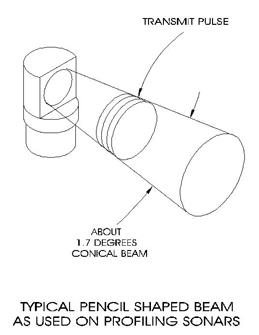
\includegraphics[width=0.5\columnwidth]{figs/sonar/3.jpg}
    \caption{T�pico feixe em formato de cone de sonares tipo \emph{profiling}}
    \label{sonar_3}
\end{figure}



 \subsubsection{Conclus�o de an�lise t�cnica}
 O ambiente no qual ser� utilizado o sonar possui uma profundidade inferior a 20 metros e a necessidade de mapeamento se localiza sobretudo em uma �rea de aproximadamente $2 \times 15$ $m^�$. Para essa situa��o o sonar profiling se mostra como o mais apropriado devido ao seu estreito feixe que otimiza a precis�o para uma pequena superf�cie pouco profunda.
 \subsubsection{Pesquisa de fornecedores}
 Os fornecedores para sonares avaliados nesta pesquisa s�o: Blueview, Echoscope, Marine Solution e Tritech. O modelo escolhido � o Super SeaKing da Tritech.


\subsection{Reconstru��o de superf�cie 3D}
%TODO retirar referencias ao Madeira

%TODO falar pq nao se pode ler dados crus
Muitos dos problemas encontrados na opera��o de inser��o e remo��o dos \textit{stoplogs} s�o provenientes da exist�ncia de objetos estranhos, trazidos pelo pr�prio rio, presentes no leito de concreto ou na superf�cie de um dos \textit{stoplogs}. A inspe��o da exist�ncia de tais objetos, isto �, a sua visualiza��o, � de suma import�ncia para que se possa determinar corretamente qual a��o corretiva � a mais apropriada.

Em ambientes subaqu�ticos onde o meio possui uma boa visibilidade, � poss�vel a utiliza��o de c�meras para a realiza��o da inspe��o. Por�m em ambientes onde a visibilidade n�o � satisfat�ria, como o caso do Rio Madeira, a utiliza��o de c�meras fica inviabilizada. Para esses casos, � necess�rio a utiliza��o de outros m�todos e sensores para a constru��o de uma representa��o 3D da superf�cie, que mapeie o ambiente com uma precis�o satisfat�ria.

Uma reconstru��o 3D de superf�cie consiste na interpreta��o e combina��o de dados, afim de se extrair informa��es tridimensionais do ambiente. Em ambientes subaqu�ticos com pouca visibilidade, o sensor recomendado para esse tipo de opera��o � o sonar. A figura \ref{figs/3d/3dcomporta} exemplifica uma reconstru��o 3D obtida pelo processamento de dados provenientes de um sonar.
\begin{figure}[H]
    \centering
    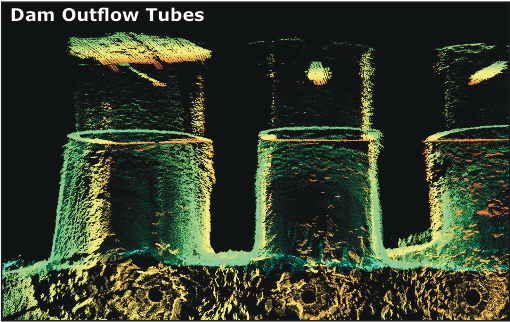
\includegraphics[width=0.9\textwidth]{figs/3d/3dcomporta}
    \caption{Exemplo de uma reconstru��o 3D da s�ida de uma barragem dos dados obtidos de um sonar 3D.}
    \label{figs/3d/3dcomporta}
\end{figure}


Um dos pontos determinantes para uma boa reconstru��o 3D � a forma de se representar e armazenar as informa��es tridimensionais, j� interpretadas dos sensores. Uma boa representa��o 3D deve possuir uma boa fidelidade do ambiente real representado, ter boa velocidade de processamento e pouca utiliza��o de mem�ria do sistema.

Ap�s a revis�o bibliogr�fica realizada, os tipos de armazenamento e representa��o mais recentes e avan�ados existentes na literatura eram a representa��o a partir de pointclouds, mapas de eleva��o e octomaps. A representa��o escolhida foi a por meio de octomaps. A seguir ser� realizado uma descri��o das principais caracter�stica de cada m�todo.
\begin{itemize}
    \item \textbf{Pointcloud} - Armazena as coordenadas tridimensionais de cada ponto lido pelo sensor. Possui uma boa fidelidade de representa��o de ambientes 3D complexos, por�m n�o � capaz de distinguir entre espa�oes vazios e ocupados.

    Por amazenar informa��es ponto a ponto, n�o possui uma eficiente utiliza��o de mem�ria. A figura \ref{fig:pointcloud} mostra a representa��o utilizando pointcloud de uma �rea externa.

    \begin{figure}[H]
    \centering
    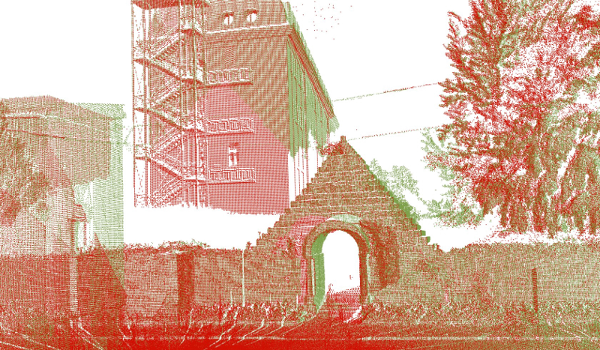
\includegraphics[width=0.8\textwidth]{figs/registration_closeup}
    \caption{Exemplo de uma reconstru��o tridimensional representado por uma Pointcloud}
    \label{fig:pointcloud}
\end{figure}


    \item \textbf{Mapas de eleva��o} - Os mapas de eleva��o representam uma superf�cie atrav�s de um grid 2D e armazenam uma informa��o de eleva��o para cada c�lula. Os mapas de eleva��o tem uma melhor efici�ncia de mem�ria, por�m para atingir essa virtude perdem o poder de representa��o fiel em todas as dimens�es. A figura \ref{fig:elevacao} mostra a representa��o utilizando mapas de eleva��o de uma �rea externa.

    \begin{figure}[H]
    \centering
    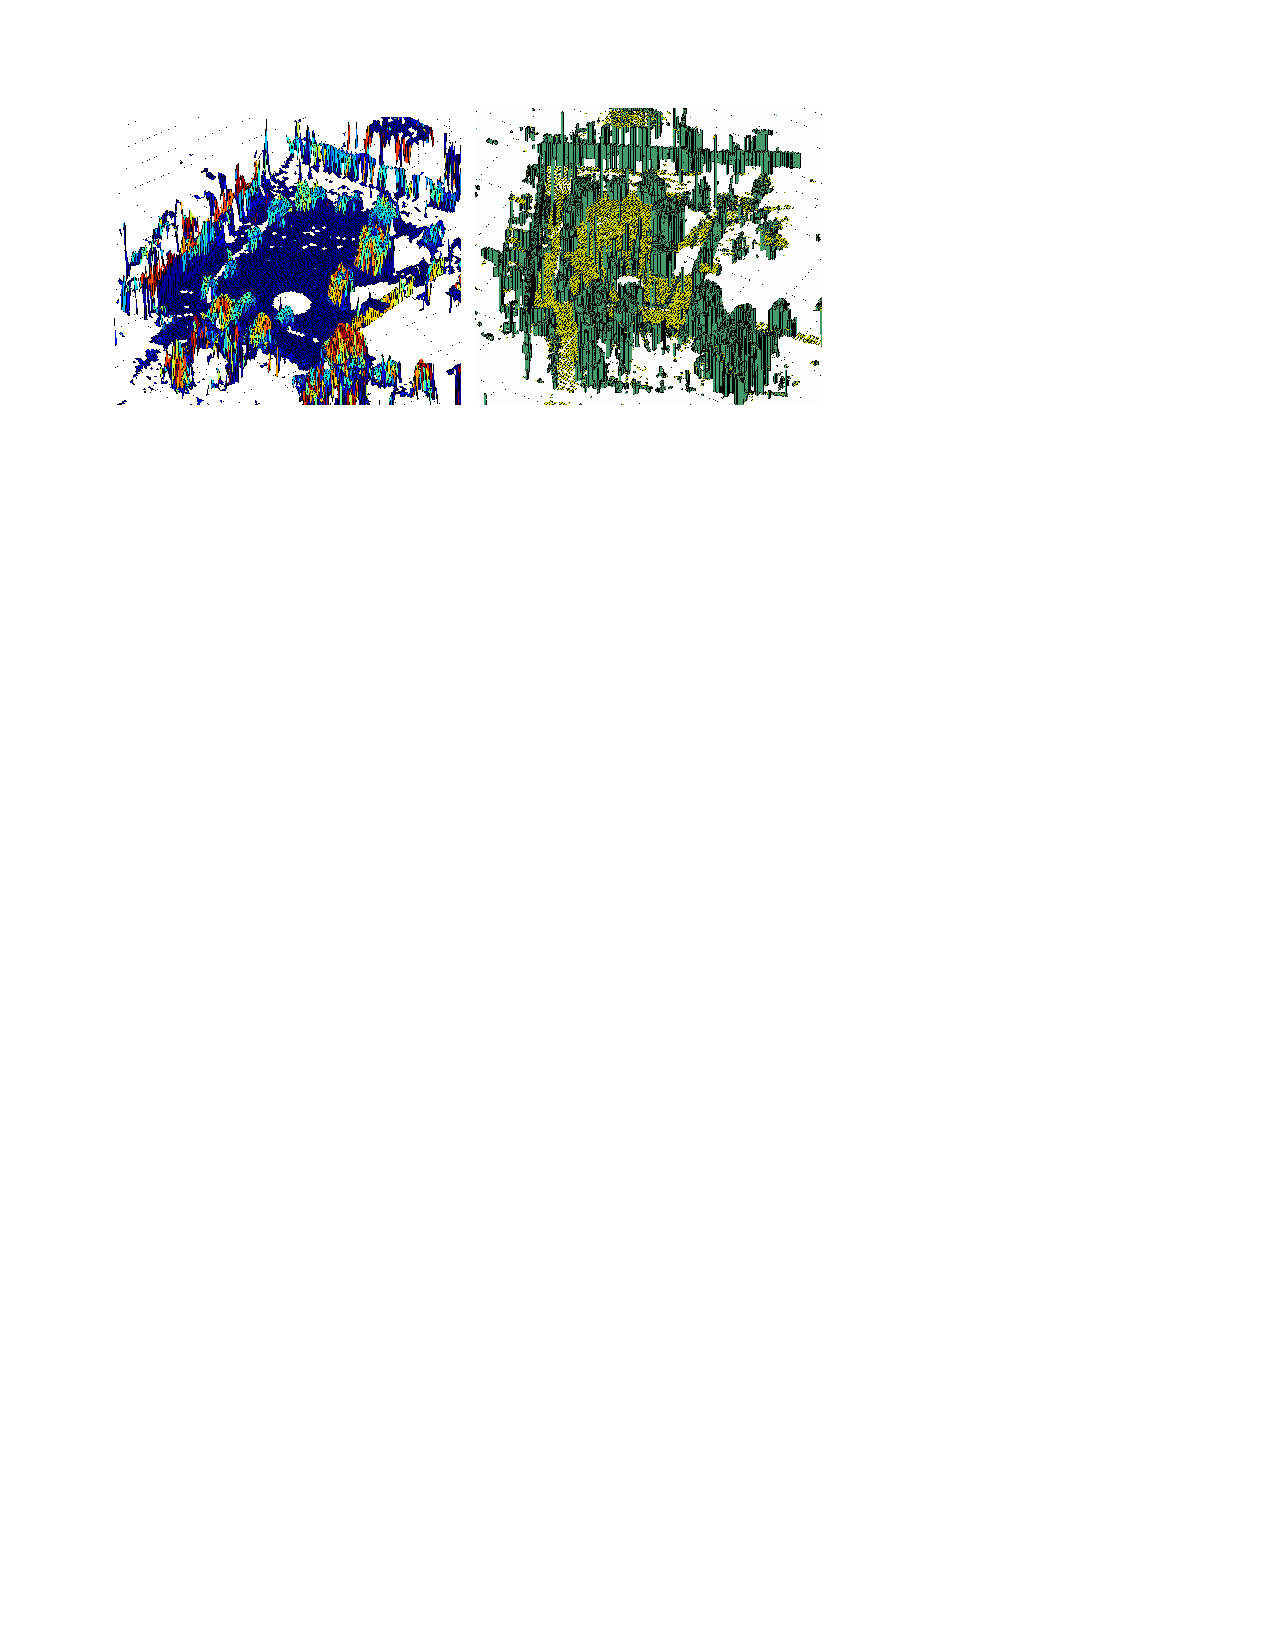
\includegraphics[width=0.8\textwidth]{figs/3d/elevationmap}
    \caption{Exemplo de uma reconstru��o tridimensional representado por um Mapa de Eleva��o}
    \label{fig:elevacao}
\end{figure}

    \item \textbf{Octomap} - Octomap � um framework livre para mapeamento 3D baseado em uma estrutura hier�rquica �rvore de dados, chamada OcTree. O espa�o tridimensional � recursivamente dividido em octantes, como exemplificado na figura \ref{fig:octree}. Aliada � estrutura de �rvore, essa caracter�stica possibilita que somente a coordenada do ponto raiz do mapa necessite ser armazenada e todas as coordenadas dos demais pontos s�o inferidas atrav�s da posi��o relativa ao ponto raiz. Diminuindo, assim, a utiliza��o de mem�ria do sistema. A estrutura hier�rquica possibilita, tamb�m, que no mapa gerado seja realizada buscas, segmenta��es para a an�lise separada de diferentes objetos e m�ltiplas resolu��es, diferentemente de mapas de resolu��o fixa como no caso da representa��o com pointclouds.

    \begin{figure}[h!]
    \centering
    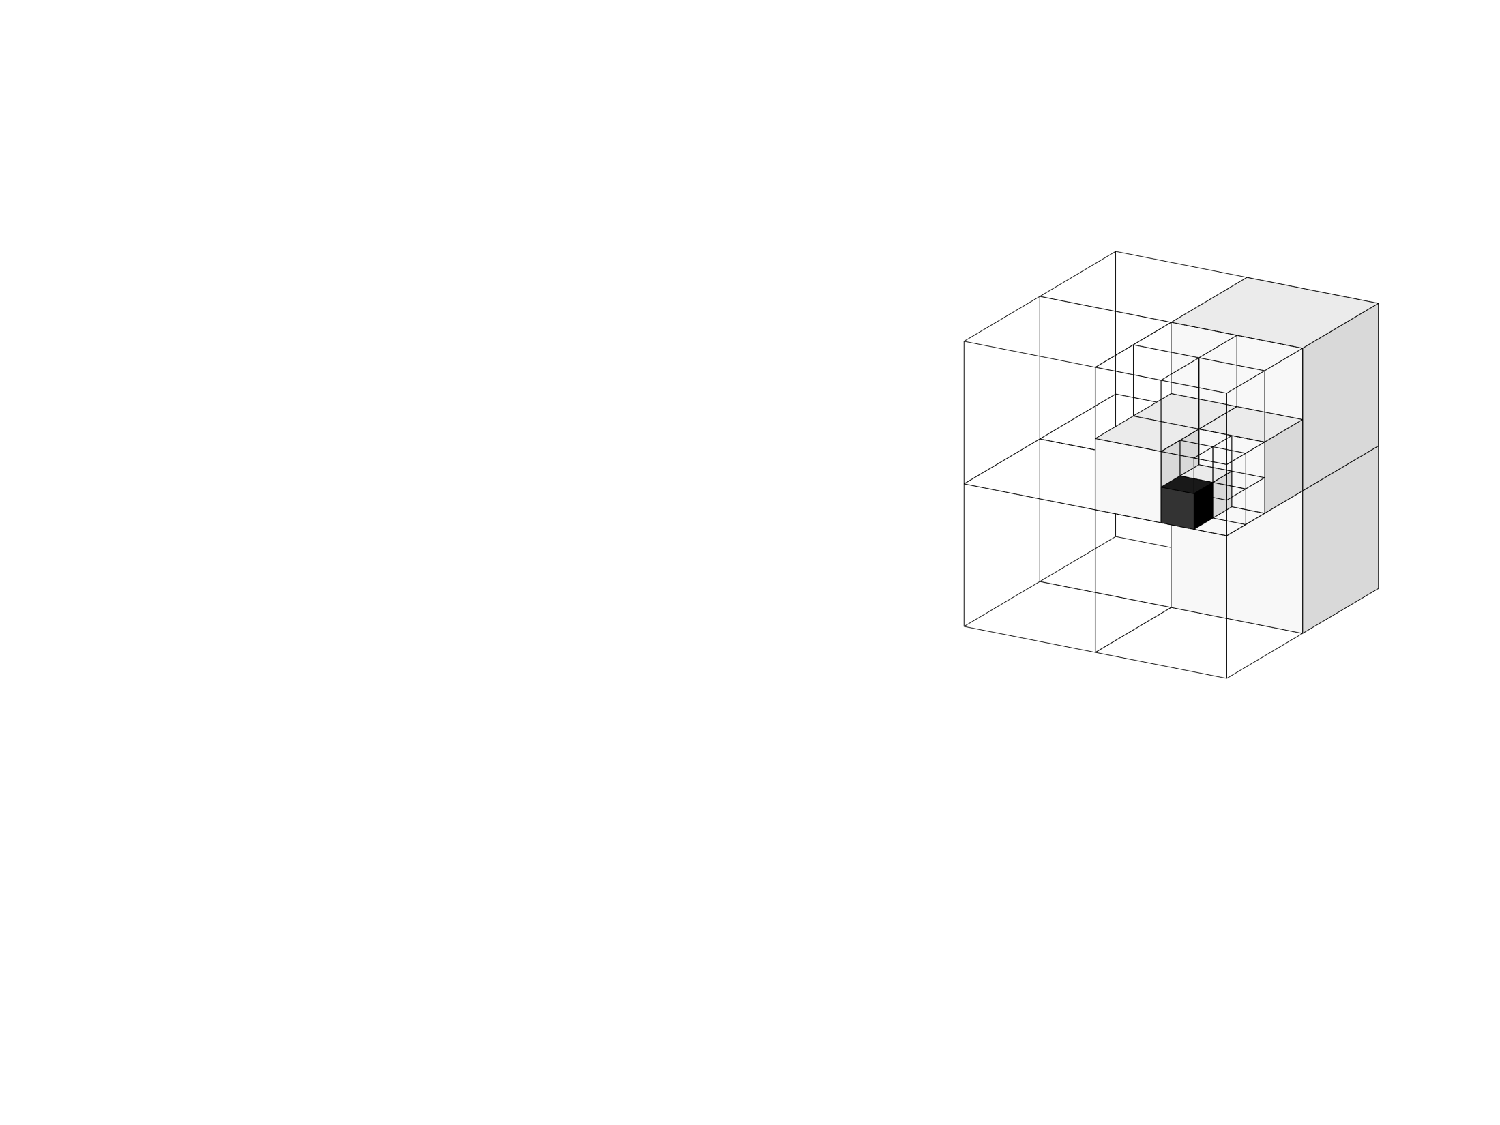
\includegraphics[width=0.4\textwidth]{figs/3d/octree}
    \caption{Divis�o recursiva do espa�o em octantes}
    \label{fig:octree}
\end{figure}
    O framework utiliza uma pol�tica de ocup�ncia probabil�stica, o que possibilita uma boa caracteriza��o de ambientes din�micos e atenua��o de ru�dos provenientes dos sensores. Outra vantagem importante � a diferencia��o de espa�os ocupados, vazios e desconhecidos, funcionalidade que n�o est� presente em nenhum dos m�todos j� apresentados. A distin��o entre espa�os que est�o desocupados e espa�os ainda n�o explorados pelo sistema  pode ser visualizada na figura \ref{fig:free} e tamb�m uma compara��o com a utiliza��o de pointclouds para o mapeamento do mesmo ambiente.

    \begin{figure}[h!]
     \centering
    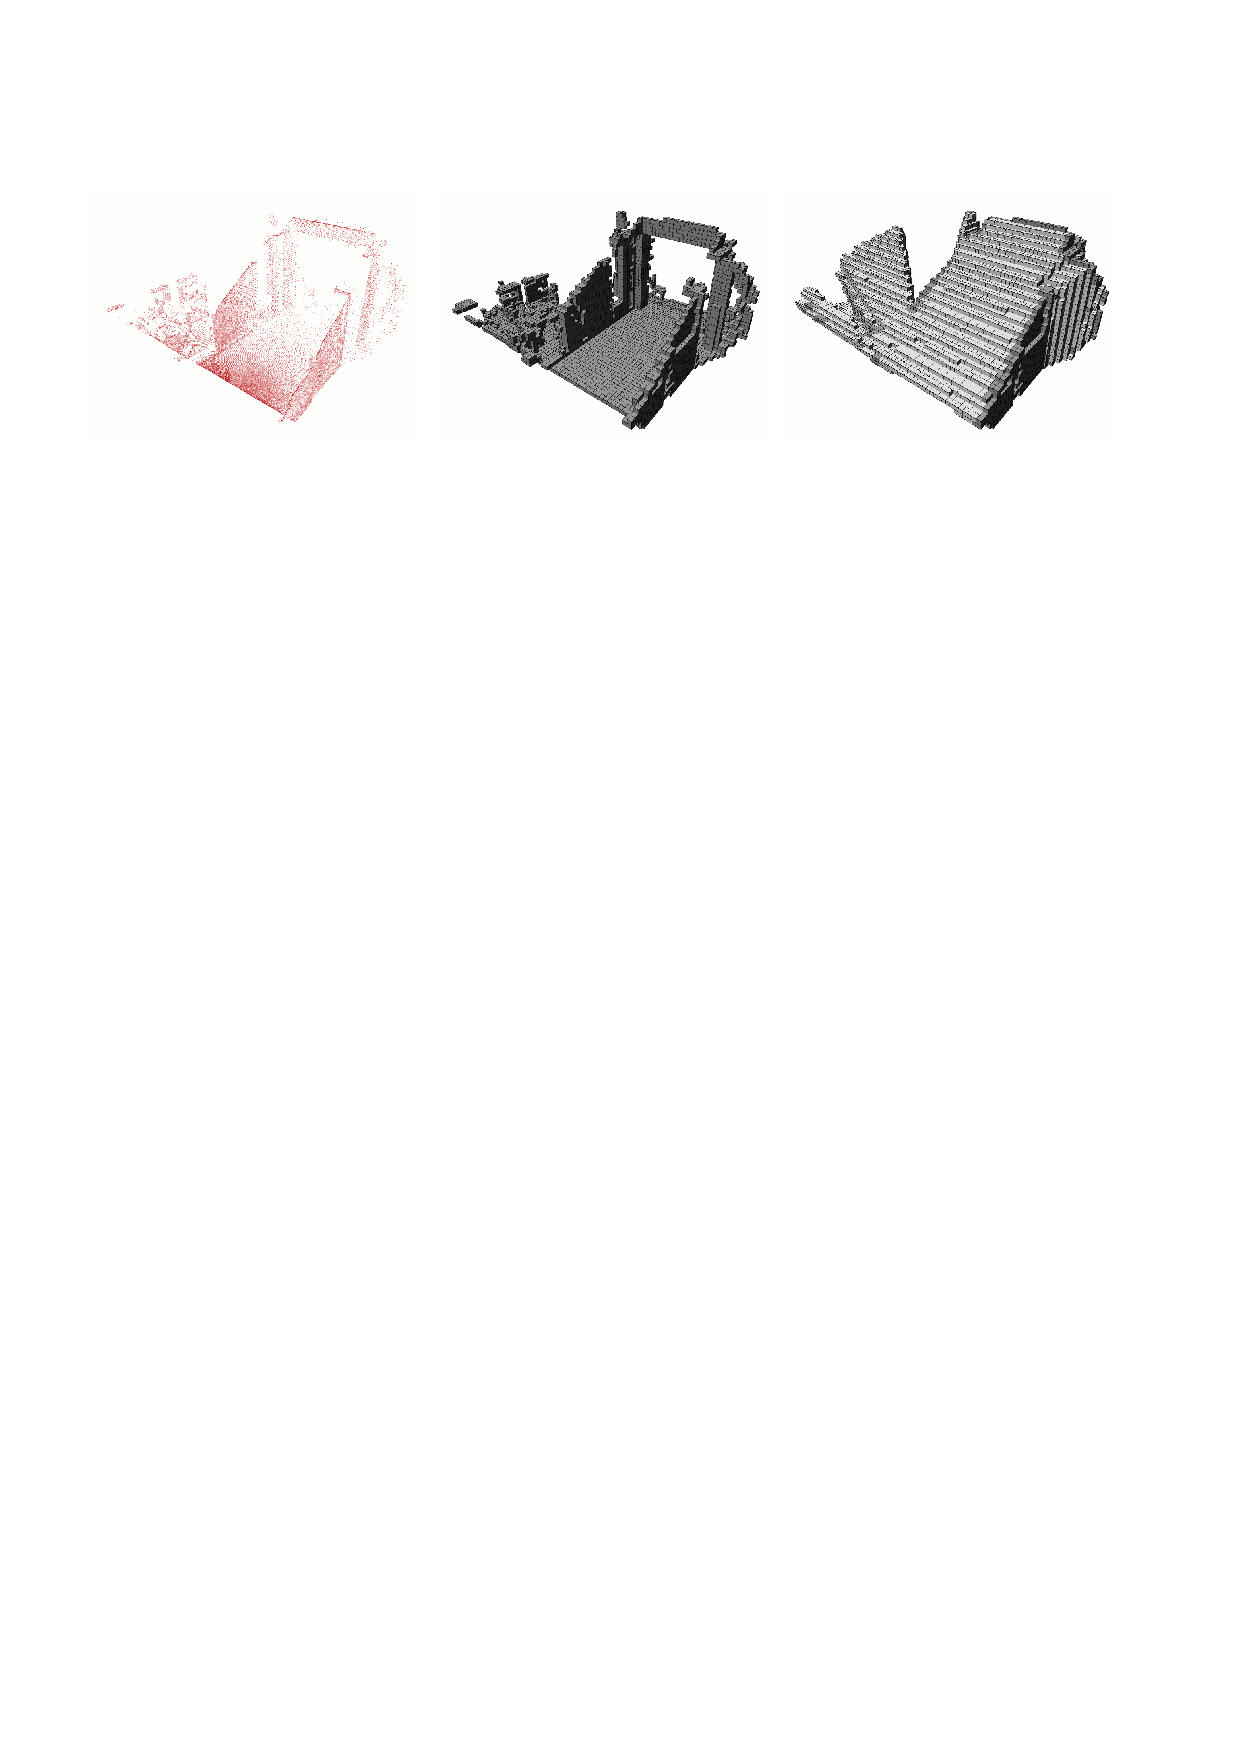
\includegraphics[width=0.95\textwidth]{figs/3d/free}
    \caption{\textit{Esquerda:} Representa��o do ambiente utilizando pointclouds e sem a possibilidade de se diferenciar espa�os desconhecidos e vazios. \textit{Meio:} Representa��o em octomap com os espa�os vazios omitidos. \textit{Direita:} Representa��o em octomap com os espa�os vazios em cinza claros e os ocupados em cinza escuro.}
    \label{fig:free}
\end{figure}
\end{itemize}

\subsubsection{Conclus�o de an�lise t�cnica}
A representa��o 3D do ambiente a ser inspecionado por meio da utiliza��o de Octomap se mostrou, al�m de mais eficiente no quesito de consumo de mem�ria, perfeitamente alinhada com as necessidades particulares da solu��o a ser proposta. A possibilidade de busca e segmenta��o do mapa, possibilita a an�lise de partes isoladas do mapa e, consequentemente, a identifica��o de objetos esperados, assim como objetos estranhos e que n�o deveriam estar presentes. A diferencia��o entre espa�os vazios e cheios e a pol�tica de ocup�ncia probabil�stica exercem uma fun��o de seguran�a, a medida que explicitam qual parte do ambiente j� foi inspecionada e atenuam poss�veis ru�dos externos e, tamb�m, intr�nsecos ao sensor.

\subsection{Sistemas de pot�ncia}
Os sistemas de pot�ncia devem ser analisados tendo em vista a opera��o convencional e excepcional. Para a opera��o excepcional, � necess�rio o uso de cabo para o fornecimento de grande pot�ncia, sendo impossibilitado o uso de bateria para esta opera��o devido � pot�ncia de opera��o da bomba. Vale notar que a pot�ncia da bomba e a consequente espessura do cabo de alimenta��o � primordial para a defini��o do carretel para esta aplica��o.

Para opera��o convencional, h� a possibilidade do uso de um outro carretel, independente do sistema de alimenta��o da bomba ou do uso de bateria e um sistema de comunica��o por ultra-som.
\subsubsection{Carretel}
Carret�is industriais s�o dispositivos para recolhimento de cabos atuados por mola. Os cabos s�o fixados e conectados em contatos girantes. Tais dispositivos apresentam robustez estrutural e resist�ncia ao tempo.

A partir da pesquisa realizada, � poss�vel concluir que h� boa disponibilidade de carret�is industriais para a aplica��o visada, inclusive com graus de prote��o adequados para umidade e resist�ncia ao tempo (NEMA4). Vale notar, portanto, necessidades essenciais para a correta especifica��o e defini��o do produto:

\begin{itemize}
  \item O local dispon�vel para fixa��o do carretel, calculando-se o comprimento ativo do cabo (a diferen�a de comprimento entre o cabo totalmente recolhido e o cabo totalmente n�o recolhido), o comprimento m�ximo suspenso do cabo e o comprimento m�ximo submerso do cabo.
	
  \item O tipo de cabo a ser utilizado, seu peso e resist�ncia � tra��o, bem como o n�mero de fios e o di�metro deste. O n�mero e expessura dos fios deve ser considerado n�o s� pelo efeito deste no peso do cabo, mas tamb�m devido � necessidade dos contatos girantes para cada condutor

  \item A op��o pelo uso de fibra �tica elimina a possibilidade de uso dos carret�is analisados, visto que n�o s� h� a quest�o de poss�veis danos � fibra devido ao enrolamento do cabo como, principalmente, h� a necessidade do uso de um acoplamento �tico girante, que n�o � disponibilizado nos carret�is analisados.
\end{itemize}

\paragraph{Conclus�o de an�lise t�cnica}\mbox{}\\
Um carretel deve ser utilizado para alimenta��o da bomba, tendo em vista a opera��o excepcional. Um segundo carretel pode ser utilizado para alimenta��o e comunica��o com o sistema eletr�nico para opera��o convencional, tendo como alternativa o uso de um sistema de bateria e de comunica��o por ultra-som.

\paragraph{Pesquisa de fornecedores}\mbox{}\\
Os fornecedores analisados que apresentam disponibilidade de carret�is adequados � aplica��o visada s�o Cavotec e Conductix. Ambas as empresas apresentam representa��o no Brasil.

\subsubsection{Bateria}
Em rela��o �s baterias, deve-se considerar sobretudo a densidade volum�trica de energia, j� que o peso n�o � uma restri��o t�o significativa na aplica��o visada.

Com a correta defini��o do tempo de opera��o e da tens�o e corrente necess�ria para o sistema, podemos definir o tipo de bateria necess�rio.

Baterias de chumbo apresentam baixa densidade energ�tica (aproximadamente 60 Wh/l) e auto-descarga em torno de 10 \% ao m�s, s�o seguras e de f�cil carga e descarga, mas t�m sua vida �til significativamente reduzida devido a aumento de temperatura.
Baterias de Ni-MH apresentam densidade de energia intermedi�ria (aproximadamente 200Wh/l). As baterias de Ni-MH convencionais apresentam auto-descarga de cerca de 30 \% ao m�s, tornando necess�ria a carga pouco tempo antes do uso, mas h� a possibilidade de utilizar baterias de Ni-MH de baixa auto-descarga (Low Self Discharge), que apresentam menor densidade de energia, mas apresentam perdas inferiores a 2\% ao m�s.

Finalmente, baterias de ion de l�tio apresentam maior densidade de energia (aproximadamente 300Wh/l) e auto-descarga de cerca de 10\% ao m�s, mas apresentam maior dificuldade de carga e a necessidade de dispositivos de prote��o, apresentam perda de carga em temperaturas mais altas e quest�es de seguran�a.

Tendo em vista tais considera��es, � razo�vel optarmos por baterias de Ni-Mh de baixa auto-descarga. Tais baterias n�o apresentam as preocupa��es de seguran�a das baterias de ion de l�tio, simplificando os sistemas de carga e de prote��o e s�o significativamente mais compactas que as baterias de chumbo.

\paragraph{Conclus�o de an�lise t�cnica}\mbox{}\\
Tendo em vista a variedade de op��es de baterias, podemos concluir que seu uso para a substitui��o de um segundo carretel ser� determinada pela disponibilidade e viabilidade do uso de um sistema de comunica��o por ultra-som.
%%******************************************************************************
%%
%% pesqbib.tex
%%
%%******************************************************************************
%%
%% Title......: Introduction
%%
%% Author.....: GSCAR-DFKI
%%
%% Started....: Nov 2013
%%
%% Emails.....: renan028@gmail.com
%%
%% Address....: Universidade Federal do Rio de Janeiro
%%              Caixa Postal 68.504, CEP: 21.945-970
%%              Rio de Janeiro, RJ - Brasil.
%%
%%******************************************************************************


%%******************************************************************************
%% SECTION - Pesquisa Técnica
%%******************************************************************************



%%%%%%%%%%%%%%

\section{Sensores de Contato}

Visando a medição do contato entre a \emph{Garra Pescadora} e o \emph{Stoplog} foram pesquisados os seguintes sistemas de sensoriamento: sensor de força, sensor indutivo de proximidade,  sensor capacitivo de proximidade. Em sequência foi realizada a
 pesquisa por fornecedores que atendam aos requisitos de projeto.
 

%%%%%%%%%%%%%%

\subsection{Sensor de força}

 Sensores de força podem ser utilizados para detectarem a presença da garra pescadora. A análise quantitativa e comparativa dessas forças pode indicar encaixe mal ou bem sucedido durante a operação e, portanto, é considerada uma solução viável mediante calibração. Os diversos tipos de sensores de força e suas aplicações podem ser consultados em \textbf{Guide to the Measurement of Force}, publicado por \textbf{The Institute of Measurement and Control, London}.

 O sensor de força é composto por um transdutor, que é submetido à força, e uma instrumentação associada, responsável por alimentar o transdutor e processar a saída. O transdutor é um dispositivo que recebe um estímulo físico, como a contração elástica do material devido ao peso, e traduz em outra medida física, como variação de voltagem ou corrente elétrica. Esta variação obedece uma relação conhecida e, dessa forma, é possível determinar quantitativamente a força aplicada.

 Existem diversos sensores de força disponíveis no mercado, com sistemas variados de operação. As principais características a serem consideradas na escolha de um sensor de força são: curva de resposta, capacidade máxima, não-linearidade, histerese, sensibilidade e reprodutibilidade.

 O sensor de força mais utilizado e que atende aos requisitos do projeto é o strain gauge. A força atua em um metal cilíndrico, que é comprimido e altera a resistência de um strain gauge, acoplado à superfície do cilindro (ver figura~\ref{forca_1}).

 \begin{figure}[H]
    \centering
    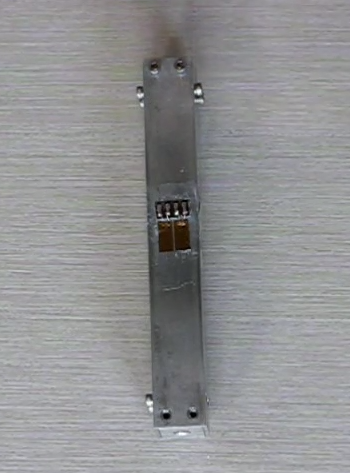
\includegraphics[width=0.4\columnwidth]{figs/forca/1.png}
    \caption{Exemplo de um sensor de força: cilindro com strain gauge acoplado.}
    \label{forca_1}
\end{figure}


 A resistência elétrica de um fio varia conforme seu comprimento e sua área, portanto, a variação de corrente que passa por este fio pode ser utilizada como medida quantitativa e é possível determinar a força aplicada por um modelo matemático conhecido: $R=\frac{\rho L}{A}$. Outros sensores que poderiam atender às especificações, mas são de mais difícil comercialização, em relação aos requisitos de projeto, são: sensor de força piezoelétrico

 De acordo com \textbf{Guide to the Measurement of Force}, a aplicação pode ser caracterizada como sistema para medições e controle de forças para operações de segurança. Pode ainda ser especificada como \textbf{Crane overload/underload protection}, que consiste em monitorar forças atuando em garras tipo pescadora ou gancho (ver figura~\ref{forca_2}), no qual a medida será avaliada em situações estáticas ou de pouco movimento/vibração.

  \begin{figure}[H]
    \centering
    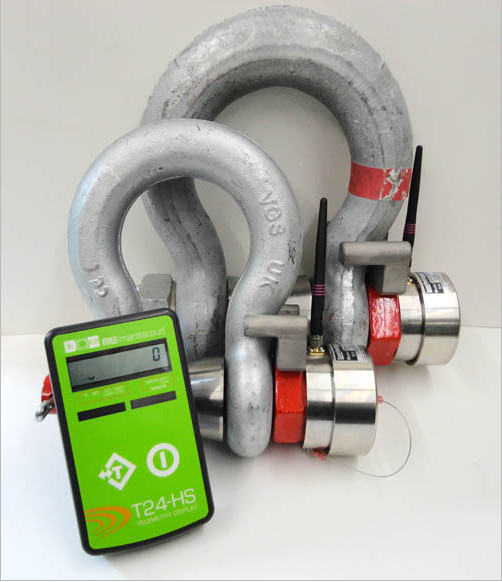
\includegraphics[width=0.4\columnwidth]{figs/forca/2.png}
    \caption{Exemplo de instalação de sensor de força em garra.}
    \label{forca_2}
\end{figure}

A solução por sensores de força é eficiente em aplicações onde se deseja avaliar frequência de vibração e duração da onda de choque, porém não muito na medida quantitativa e comparativa de forças devido à sensibilidade do strain gauge a campos magnéticos externos, pressão hidrostática e umidade. A variação de acúmulo de sedimentos no stoplog também dificulta a calibração do instrumento.

Os fornecedores para sensores de força do tipo strain gauge avaliados nesta pesquisa são: Applied Measurements Limited, Load Cell Central, Transducer Techniques. Os modelos avaliados são da série DBEP e CLP de seus respectivos fornecedores.


%%%%%%%%%%%%%%

\subsection{Sensor indutivo de proximidade}

Sensores indutivos de proximidade podem ser utilizados para detectarem a presença da garra pescadora. Este sensor de presença pode ser do tipo linear, podendo ser realizada análise quantitativa, ou simplesmente chaveado, um simples indicador de presença. Portanto, pode indicar encaixe mal ou bem sucedido durante a operação de remoção/inserção de stoplogs. Os sensores indutivos apresentam a mesma forma de operação nos diversos produtos disponíveis no mercado, diferenciando-se principalmente na medida de distância da aplicação.

 O sistema para sensoriamento por indução magnética é composto por uma fonte de alimentação e um indutor. Ao alimentar o sensor indutivo, uma corrente alternada é gerada. A corrente elétrica que passa pelo indutor gera um campo magnético na face do sensor. Este campo magnético induz corrente de Foucault no alvo metálico, que aumenta conforme o alvo se aproxima do sensor indutivo. O aumento das correntes de Foucault cria um campo magnético no alvo, que irá se opor ao campo produzido pelo sensor indutivo. Essa redução do campo magnético pode ser medida e, portanto, é possível presenciar o alvo.

 Existem diversos sensores indutivos disponíveis no mercado que atendem às especificações, apresentam o mesmo modo de operação e diferenciam-se principalmente quanto à robustez, instalação (faceada ou não) e interface de saída. A resistência a choques, vibração, submersibilidade e o tipo de instalação são as características mais importantes para a aplicação. O sensor deve ser do tipo IP69K e faceado, o que diminui o alcance, mas aumenta a proteção.

 A pesquisa por sensores indutivos de proximidade para a finalidade desejada resultou em aplicações equivalentes. A empresa \textbf{HATCH - Energy Innovations} desenvolveu em 2007 um Lifting Beam instrumentado com sensores indutivos (ver figura~\ref{indutivo_1}). Em 2008, a empresa \textbf{Atlas Polar} adotou a mesma solução com sensores indutivos.

 \begin{figure}[H]
    \centering
    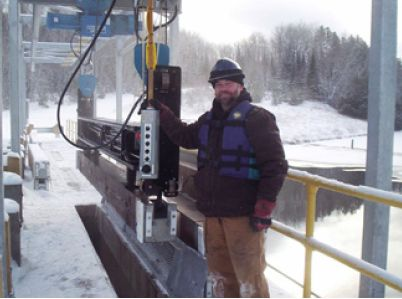
\includegraphics[width=0.5\columnwidth]{figs/indutivo/1.jpg}
    \caption{Lifting Beam desenvolvido pela empresa HATCH}
    \label{indutivo_1}
\end{figure}

A solução por sensores indutivos é eficiente em aplicações onde se deseja avaliar a presença de stoplog. A grande maioria dos sensores são frágeis a choque e vibração, além de sensíveis a ruídos elétricos e magnéticos. Porém, já há no mercado produtos IP69K e encapsulados. Há, também, a possibilidade de falso positivo em caso de sedimentos metálicos, mas é baixa a probabilidade.
Pesquisas em aplicações semelhantes mostraram que o sensor indutivo é a solução adotada para o monitoramento de encaixe entre garra pescadora e stoplog, auxiliado por outros sensores ou sistemas independentes de atuadores.

Os fornecedores pesquisados para sensores indutivos que atendem aos requisitos de projeto são: Contrinex, Pepperl-Fuchs, Positek e Turck. Diversos modelos foram avaliados, juntamente com os técnicos das respectivas empresas.

%%%%%%%%%%%%%%

\subsection{Sensor capacitivo de proximidade}
Os sensores capacitivos de proximidade são capazes de detectar objetos devido à capacidade destes alvos em serem carregados eletricamente. Analogamente ao sensor indutivo, que detecta variações de campo magnético devido a alvos metálicos, o sensor capacitivo é sensível a variações na capacitância (ver figura~\ref{capacitivo_1}).

\begin{figure}[H]
    \centering
    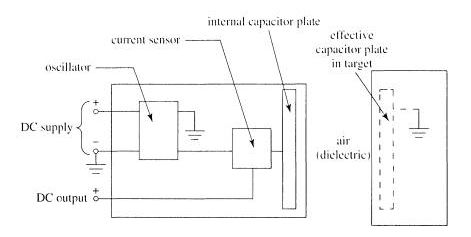
\includegraphics[width=0.8\columnwidth]{figs/capacitivo/1.jpg}
    \caption{Sensor capacitivo}
    \label{capacitivo_1}
\end{figure}

Internamente ao sensor, há um circuito que utliza a alimentação DC para gerar voltagem alternada (oscilador). O circuito interno RC é, então, alimentado e uma corrente alternada passa por esse circuito. O fluxo de corrente alternada depende da capacitância, e esta varia  conforme a distância e área entre as placas do capacitor e o material dielétrico entre as placas: $C = \frac{\epsilon A}{d}$.

Em sensores capacitivos, uma placa do capacitor está no sensor e a outra é o objeto a ser detectado, que pode ser um material metálico ou não-metálico. A aproximação do alvo modifica a capacitância, resultando em variações no campo elétrico e na corrente alternada. Finalmente, as variações da corrente podem ser medidas e o alvo é detectado.

As características que devem ser avaliadas em sensores capacitivos são as mesmas dos sensores indutivos, como tipo de instalação, modo de operação chaveado ou linear e etc. Porém, deve-se atentar ao fator de redução, que depende do alvo a ser detectado.

 Os sensores capacitvos exercem função semelhante ao sensor indutivo e pode ser utilizado para detecção de presença de stoplog. Porém, a calibração se mostra bem mais complexa devido à sensibilidade do sensor e ao fato de não estar restrito a detecção de materiais metálicos. A chance de falsos positivos será bem maior em caso de escolha deste sensor em comparação com o sensor indutivo.


Os fornecedores pesquisados de sensores capacitivos que atendem aos requisitos de projeto são: Contrinex, Pepperl-Fuchs, Positek e Turck. Diversos modelos foram avaliados, juntamente com os técnicos das respectivas empresas.

%% ***************


 \subsection{Conclusão de análise técnica}\mbox{}\\


As tecnologias que foram analisadas para detectar o contato entra a garra pescadora e o Stoplog foram: sensor de força, sensor indutivo e sensor capacitivo. Os sensores de força necessitaria de ser instalados nos eixos da garra pescadora, logo alterando a estrutura mecânica do mesmo, além de serem sensíveis a calibração, logodesconsiderados como uma solução viável. O sensor capacitivo, assim como o sensor indutivo, podem ser instalados diretamente na garra pescadora, entretanto o capacitivo não está restrito a detecção de materiais metálicos, logo resultaria em maiores chances de falsos positivos que os sensores indutivos.  Sendo assim, a solução de medição de contato por sensor indutivo se mostra mais eficiente para a detecção do contato entre a garra pescadora e o Stoplog. 

Dados os requerimentos do meio foi buscado no mercado produtos a prova d’agua e encapsulados com nível de proteção mínima IP69K. Os fornecedores pesquisados para sensores indutivos que atendem aos requisitos de projeto são: Contrinex, Pepperl-Fuchs, Positek e Turck. Diversos modelos foram avaliados, juntamente com os técnicos das respectivas empresas. A lista dos modelos de cada fabricante que seriam ideais à aplicação no projeto se encontra na tabela abaixo. Por os modelos serem equivalente em aplicabilidade, foi selecionado o sensor que apresenta o menor custo ao projeto o NBB20-L2-E2-V1 de instalação faceada, chaveado normalmente aberto e distância de operação de 2cm (figura~\ref{indutivo_1}).


\begin{center}
    \begin{tabular}{| l | l | l | l | }
    \hline
	{\bf Modelo} & 	{\bf Fabricante} &		{\bf Distribuidor}	&	{\bf Preço} \\  \hline
	DW-LD-M18&		Contrinex&			Electric Control&		428,97 R{\$} \\  \hline
	NBB20&			Pepperl-Fuchs&		Pepperl-Fuchs Brasil&	181,17 R{\$} \\  \hline
	NI35&			TURCK&				TURCK Brasil&			514,29 R{\$} \\  \hline
	NI50-Q42&		TURCK&				TURCK Brasil&			414,75 R{\$} \\ \hline
\hline 
\end{tabular}
\end{center}

\begin{figure}[H]
    \centering
    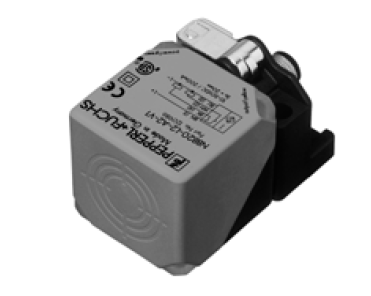
\includegraphics[width=0.4\columnwidth]{figs/indutivo/1.png}
    \caption{Sensor indutivo do fornecedor Pepperl-Fuchs.}
    \label{indutivo_1}
\end{figure}
%%******************************************************************************
%%
%% pesqbib.tex
%%
%%******************************************************************************
%%
%% Title......: Introduction
%%
%% Author.....: GSCAR-DFKI
%%
%% Started....: Nov 2013
%%
%% Emails.....: renan028@gmail.com
%%
%% Address....: Universidade Federal do Rio de Janeiro
%%              Caixa Postal 68.504, CEP: 21.945-970
%%              Rio de Janeiro, RJ - Brasil.
%%
%%******************************************************************************


%%%%%%%%%%%%%%%%%%%%%%%%%%%%%%
%%%%%%%%%%%%%%%%%%%%%%%%%%%%%%

\section{Posição Angular}

O Sistema de Lifting Beam desenvolvido em aplicação semelhante de remoção e inserção de stoplogs pela empresa \textbf{HATCH} utliza atuadores elétricos independentes em cada garra, o que permite o monitoramento da abertura das garras, sendo possível saber quando há encaixe mal ou bem sucedido. O sistema em estudo a ser desenvolvido, porém, é a monitoramento de um Lifting Beam mecânico, onde as garras abrem e fecham passivamente. Por questões de restrição de projeto, não é permitido alterar a estrutura mecânica de forma que as garras sejam atuadas independentemente, mas é permitida a instrumentação do Lifting Beam com encoders, sendo possível instalá-los nas vigas das garras, a fim de medir suas posições angulares. A movimentação angular das garras durante o encaixe é conhecido e sequencial, de forma que uma simples anlálise comparativa com os dados fornecidos pelos encoders durante a execução da tarefa pode indicar se o encaixe foi mal ou bem sucedido.

\subsection{Encoder}
O encoder óptico é um dispositivo eletromecânico que entrega como saída um sinal elétrico proporcional à posição angular do eixo acoplado. O eixo é acoplado mecanicamente a um disco opaco e marcado em sua superfície por segmentos (ver figura~\ref{encoder_1}).

\begin{figure}[H]
    \centering
    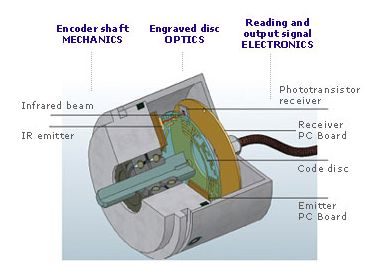
\includegraphics[width=0.5\columnwidth]{figs/encoder/1.jpg}
    \caption{Sistema interno de um encoder.}
    \label{encoder_1}
\end{figure}

Diodos emissores de luz infravermelha alcança os receptores através das fendas do disco. O sinal analógico é criado, amplificado, convertido em digital e transmitido ao processador.

Além dos requisitos básicos do projeto, como submersibilidade e resistência a choque e vibração, as principais características a serem avaliadas neste projeto para a escolha de um encoder são: modo de operação incremental ou absoluto, multi-voltas ou não, interface de comunicação, resolução e tensão de operação.

 \subsection{Conclusão de análise técnica}
A pesquisa mostrou ampla aplicação de encoders para a aplicação e é esperado que seja possível identificar encaixe mal ou bem sucedido com sua utielização. A instalação do encoder na viga da garra pescadora não é mecanicamente complexa e não resultará em alteração permanente da estrutura.


Os fornecedores para encoders que atendem aos requisitos de projeto pesquisados são: Hohner, IFM, Pepperl-Fuchs e Rotary Encoder Solutions. O modelo selecionado, após ampla análise entre fornecedores, é o
modelo Encoder RM9000 Absoluto com interface CAN, multi-voltas que apresenta a configuração necessária para a aplicação e o menor custo para o projeto dentro os modelos analisados. 
(figura~\ref{encoder_1})

SUBXWD	Hohner	Hohner Brasil	R$ 3.248,91
AR63	Rotary Encoder Solutions	-	R$ 2.949,61
CVS42H	Pepperl-Fuchs	Pepperl-Fuchs Brasil	R$ 2.586,46
RM9000	IFM	IFM Brasil	R$ 1.298,69

\begin{center}
    \begin{tabular}{| l | l | l | l | }
    \hline
	{\bf Modelo} 	& 	{\bf Fabricante} 	&		{\bf Distribuidor}	&	{\bf Preço} \\  \hline
	SUBXWD&			Hohner&					Hohner Brasil&			 3.248,91 R{\$} \\  \hline
	AR63&			Rotary Encoder Solutions	&	-&					2.949,61 R{\$} \\  \hline
	CVS42H&			Pepperl-Fuchs&			Pepperl-Fuchs Brasil&	2.586,46 R{\$} \\  \hline
	RM9000&			IFM&						IFM Brasil&			1.298,69 R{\$} \\ \hline
\hline 
\end{tabular}
\end{center}

\begin{figure}[H]
    \centering
    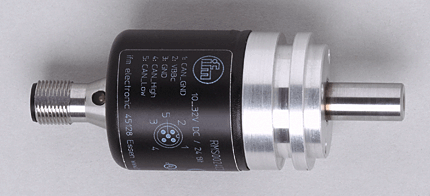
\includegraphics[width=0.4\columnwidth]{figs/encoder/1.png}
    \caption{Encoder do fornecerdor IFM}
    \label{encoder_1}
\end{figure}


\subsection{Mapeamento 3D}

Muitos dos problemas encontrados na operação de inserção e remoção dos
\textit{stoplogs} são provenientes da existência de objetos estranhos, trazidos
pelo próprio rio, presentes no leito de concreto ou na superfície de um dos
\textit{stoplogs}. A inspeção da existência de tais objetos, isto é, a sua
visualização, é de suma importância para que se possa determinar corretamente
qual ação corretiva é a mais apropriada.

Em ambientes subaquáticos onde o meio possui uma boa visibilidade, é possível a
utilização de câmeras para a realização da inspeção. Porém em ambientes onde a
visibilidade não é satisfatória, a utilização de câmeras fica inviabilizada.
Para esses casos, é necessário a utilização de Sonares para a
visualização do ambiente a ser inspecionado. Porém os Sonares utilizados para
mapear os ambientes não tem uma resposta que é facilmente interpretada pelo ser
humano e, por isso, é necessário que se faça uma conversão dos dados e uma a
construção de uma representação 3D da superfície.

Nesta secção será apresentado o que é o sensor Sonar e determinando através de uma análise técnica e de fornecedores qual o Sonar que atende aos requisitos de projeto. Assim como, será descrito qual tecnologia de mapeamento 3D será aplicada ao projeto. 



\subsubsection{Sonar}
Sonar\footnote{A sigla tem origem como acrônimo de \textit{sound navigation and ranging}.} é uma técnica que utiliza a propagação do som na água para se comunicar e detectar objetos nesse meio, ela possui duas vertentes uma chamada ativa e outra passiva. A passiva se resume a escutar o meio e não será investigada, pois não possui a funcionalidade para o mapeamento de superfícies submersas. Os equipamentos que fazem uso de tal tecnologia acabam por herdar seu nome, assim sonares que utilizam a tecnologia ativa são chamados de sonares ativos.

O sonar ativo, daqui em diante apenas referido como sonar, emite um ping que é um pulso de onda sonora que será refletido pelo meio. Conforme a frente de onda atravessa os objetos submersos ela é refletida e este eco é detectado no retorno pelo sonar, onde ele extrai as informações do tempo que a onda levou para retornar e sua intensidade, podendo, a partir do conhecimento de características do meio, como a velocidade de propagação do som, estimar a distancia de origem do eco e consequentemente do objeto.

Pela aplicação os sonares são divididos em basicamente duas categorias: \emph{profiling} e \emph{imaging};

O sonar do tipo \emph{imaging} são tipicamente utilizados para fazer o mapeamento do fundo do mar, possuindo uma abertura em formato de leque (ver figura~\ref{sonar_1}), eles podem utilizar um motor de rotação sobre o eixo perpendicular ao feixe ou podem ser arrastados pela água para fazer o escaneamento (ver figura~\ref{sonar_2}).

\begin{figure}[H]
    \centering
    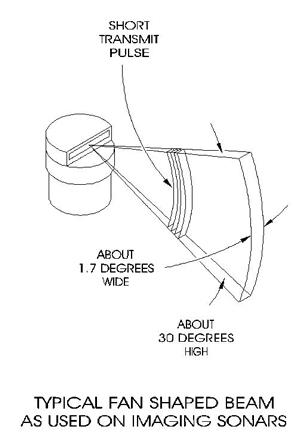
\includegraphics[width=0.5\columnwidth]{figs/sonar/1.jpg}
    \caption{Típico feixe em formato de leque de sonares tipo \emph{imaging}}
    \label{sonar_1}
\end{figure}

\begin{figure}[H]
    \centering
    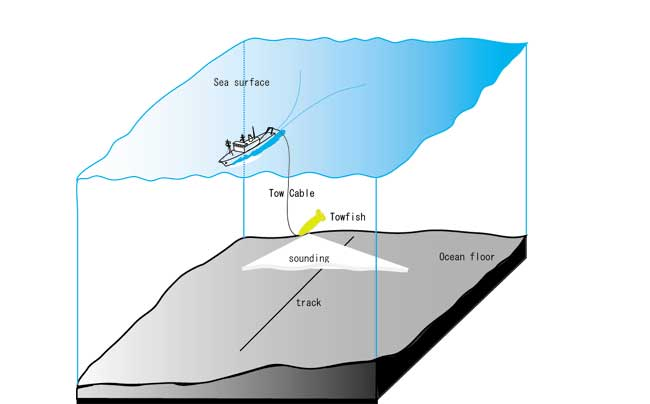
\includegraphics[width=0.5\columnwidth]{figs/sonar/2.jpg}
    \caption{Sonar \emph{imaging} sendo arrastado para mapeamento das profundezas}
    \label{sonar_2}
\end{figure}


A resposta dos sonares tipo \emph{imaging} forma uma imagem colorida exibindo tons diferentes para respostas mais fortes e mais fracas de eco do sonar. Sendo utilizado para obter uma imagem do fundo do mar semelhante as que os radares fazem na superfície.

Pela tecnologia empregada os sonares \emph{imaging} possuem dois tipos de configuração: \emph{multibeam} e \emph{mechanical} (single beam).

A configuração \emph{single beam} possui um transdutor acoplado a um mecanismo de \emph{pan} para possibilitar a varredura de determinada área. Assim, o sonar envia seu \emph{ping} espera o eco de retorno e avança para a próxima posição determinada pelo passo, ou resolução angular, do motor que compõe o mecanismo de \emph{pan}.

Alternativamente, os sonares \emph{multibeam} possuem idealmente um feixe \emph{ping} extremamente amplo, sendo na prática composto por diversos feixes com seus respectivos transdutores sincronizados. Essa configuração possui diversos receptores espalhados por uma região do sonar, resolvendo qual a posição de origem do eco através de um sistema de multilateração. Assim, o \emph{multibeam} sobrepuja a configuração \emph{single beam} no aspecto de precisão e tempo de varredura.

De forma diferente, os sonares do tipo \emph{profiling} retornam apenas um valor e não uma graduação de tons. Esse valor é referente, normalmente, ao tempo de retorno do eco mais intenso dentro do intervalo de amostragem, intervalo de espera que delimita o alcance máximo de interesse. Esses sonares também podem ser configurados para enviarem o valor do tempo de retorno do primeiro eco, em vez do mais intenso, de maneira a agilizar o processo de captura de dados, pois todos os ecos à partir do primeiro são ignorados, passando para a emissão de um novo \emph{ping} em uma nova posição.

Outra característica importante dos sonares \emph{profiling} é o formato do seu feixe, este possui uma abertura estreita de formato tipicamente cônico (ver figura~\ref{sonar_3}).

\begin{figure}[H]
    \centering
    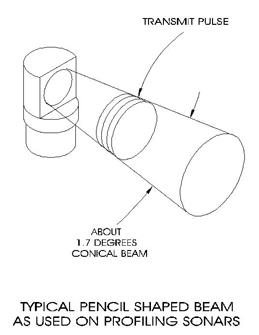
\includegraphics[width=0.5\columnwidth]{figs/sonar/3.jpg}
    \caption{Típico feixe em formato de cone de sonares tipo \emph{profiling}}
    \label{sonar_3}
\end{figure}

A figura \ref{sonar_4}) demonstra comparativamente a diferença entre os diferentes tipos de sonares.

\begin{figure}[H]
    \centering
    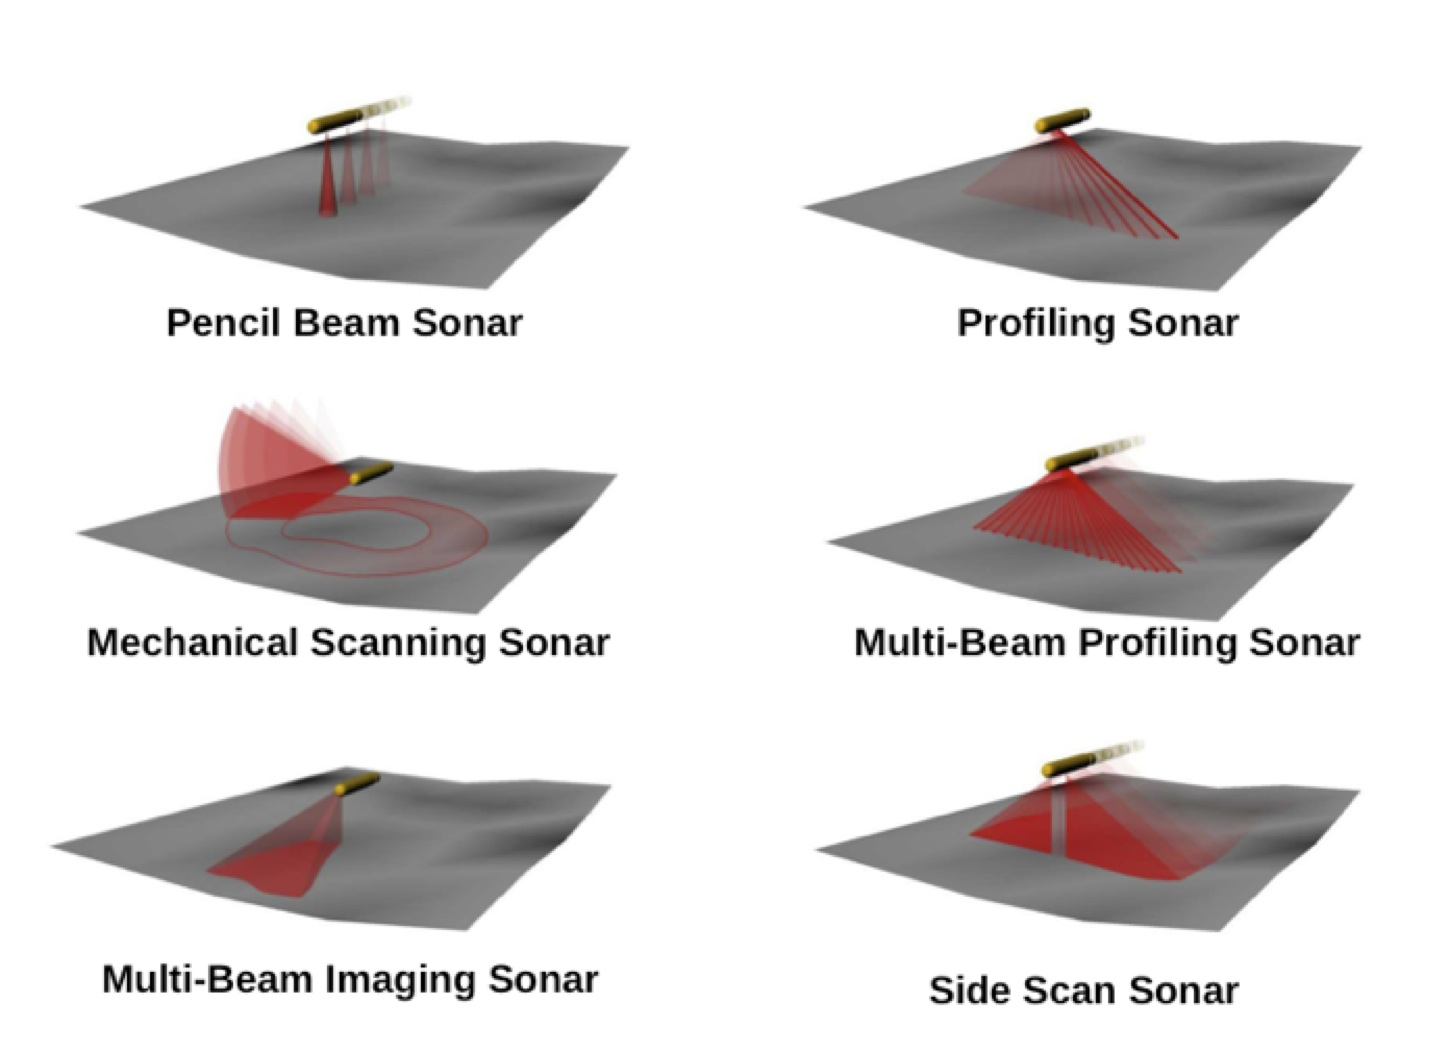
\includegraphics[width=1\columnwidth]{figs/sonar/4.jpg}
    \caption{Tipos de Sonares}
    \label{sonar_4}
\end{figure}


 \paragraph{Conclusão de análise técnica}\mbox{}\\
 O ambiente no qual será utilizado o sonar possui uma profundidade inferior a 20
 metros e a necessidade de mapeamento se localiza sobretudo em uma área de
 aproximadamente $2 \times 15 m^2$. Para essa situação o sonar profiling se
 mostra como o mais apropriado devido ao seu estreito feixe que otimiza a
 precisão para uma pequena superfície pouco profunda. 

Os fornecedores e modelos pesquisados estão apresentados na tabela abaixo. Dentre os modelos análisados o Super Seaking DFP e Micron apresentam o melhor custo. A diferença de custo entre ambos os modelos se dá devido a diferença da abertura do feixe. O Super Seaking DFP possui um feixe mais estreito, o que permite uma maior precisão. Não é possível determinar qual seria o modelo mais aplicável apenas por análise teória, logo parte da pesquisa deste projeto será testar ambos os modelos para determinar qual é o mais aplicável.  


\begin{center}
    \begin{tabular}{| l | l | l | l | }
    \hline
	{\bf Modelo} & 	{\bf Fabricante} &		{\bf Distribuidor}	&	{\bf Preço} \\  \hline
	BV5000 &			Blueview&				- &					323.000,40R{\$} \\  \hline
	3D Echoscope&	Octopus&		 		Seatronics&			960.000,00 R{\$} \\  \hline
	DT101&			Imagenex&			Marine Solution&	365.000R{\$} \\  \hline
	Super Seaking DFP&		Tritech&				MacSea&			33.990,50R{\$} \\ \hline
	Micron Sonarg &		Tritech&				MacSea&			16.798,90R{\$} \\ \hline

\hline 
\end{tabular}
\end{center}


\subsubsection{Unidade Pan e Tilt}

O sonar tipo profiling definido possui apenas 1 grau de liberade interno, logo não é possível mapear toda a região do trilho do stoplog com o mesmo a partir de uma posição fixa de acoplamento na garra pesacdora. Logo, uma unidade de pan e tilt será acoplado ao Sonar possibilitando assim cobrir toda a extensão do trilho do Stoplog. 

O fator mais importante na escolha do motor de posicionamento é a precisão que o mesmo consegue operar, pois o sonar mede a distância ao meio que se encontra de 3 a 50 metros de distância do mesmo, logo um pequeno erro de posicionamento angular do motor resultará em um erro grande na reconstrução do meio. Exemplo: 1 grau de erro a 50m de distância significaria 0,87m de erro na reconstrução do ambiente. A tabela abaixo lista alguns dos modelos disponíveis no mercado, sua precisão dada a folga mecânica do mesmo e o custo.  Logo, o modelo escolhido para o projeto foi o OE10-102 da Kongsberg que oferece a menor folga mecânica.

\begin{center}
    \begin{tabular}{| l | l | l | l | }
    \hline
	{\bf Modelo} & 	{\bf Fabricante} &		{\bf Folga}	&	{\bf Preço} \\  \hline
	PT-10FB &			ROS&				0.6deg &		24.101,90 R{\$} \\  \hline
	SS109&				Sidus&				 0.5deg&			14.576,57 R{\$} \\  \hline
	OE10-102&			Kongsberg&			0.08 def&	 		29.441,40 R{\$} \\  \hline

\hline 
\end{tabular}
\end{center}

%%%%%%%%%%%%%%%%%%%%%%%%%%%%%%%%%%%%%%%%%%%%%%%%%%%%%%%%%%%%%%%%%%%%%%%%%%

\subsection{Reconstrução de superfície 3D}

Uma reconstrução 3D de superfície consiste na interpretação e combinação de
dados, afim de se extrair informações tridimensionais do ambiente. Em ambientes
subaquáticos com pouca visibilidade, o sensor recomendado para esse tipo de
operação é o sonar. A figura \ref{figs/3d/3dcomporta} exemplifica uma
reconstrução 3D obtida pelo processamento de dados provenientes de um sonar.
\begin{figure}[H]
    \centering \includegraphics[width=0.9\textwidth]{figs/3d/3dcomporta}
    \caption{Exemplo de uma reconstrução 3D da sáida de uma barragem dos dados obtidos de um sonar 3D.}
    \label{figs/3d/3dcomporta}
\end{figure}


Um dos pontos determinantes para uma boa reconstrução 3D é a forma de se representar e armazenar as informações tridimensionais, já interpretadas dos sensores. Uma boa representação 3D deve possuir uma boa fidelidade do ambiente real representado, ter boa velocidade de processamento e pouca utilização de memória do sistema.

Após a revisão bibliográfica realizada, os tipos de armazenamento e representação mais recentes e avançados existentes na literatura eram a representação a partir de pointclouds, mapas de elevação e octomaps. A representação escolhida foi a por meio de octomaps. A seguir será realizado uma descrição das principais característica de cada método.
\begin{itemize}
    \item \textbf{Pointcloud} - Armazena as coordenadas tridimensionais de cada ponto lido pelo sensor. Possui uma boa fidelidade de representação de ambientes 3D complexos, porém não é capaz de distinguir entre espaçoes vazios e ocupados.

    Por amazenar informações ponto a ponto, não possui uma eficiente utilização de memória. A figura \ref{fig:pointcloud} mostra a representação utilizando pointcloud de uma área externa.

    \begin{figure}[H]
    \centering
    \includegraphics[width=0.8\textwidth]{figs/3d/registration_closeup}
    \caption{Exemplo de uma reconstrução tridimensional representado por uma Pointcloud}
    \label{fig:pointcloud}
\end{figure}


    \item \textbf{Mapas de elevação} - Os mapas de elevação representam uma superfície através de um grid 2D e armazenam uma informação de elevação para cada célula. Os mapas de elevação tem uma melhor eficiência de memória, porém para atingir essa virtude perdem o poder de representação fiel em todas as dimensões. A figura \ref{fig:elevacao} mostra a representação utilizando mapas de elevação de uma área externa.

    \begin{figure}[H]
    \centering
    \includegraphics[width=0.8\textwidth]{figs/3d/elevationmap}
    \caption{Exemplo de uma reconstrução tridimensional representado por um Mapa de Elevação}
    \label{fig:elevacao}
\end{figure}

    \item \textbf{Octomap} - Octomap é um framework livre para mapeamento 3D baseado em uma estrutura hierárquica árvore de dados, chamada OcTree. O espaço tridimensional é recursivamente dividido em octantes, como exemplificado na figura \ref{fig:octree}. Aliada à estrutura de árvore, essa característica possibilita que somente a coordenada do ponto raiz do mapa necessite ser armazenada e todas as coordenadas dos demais pontos são inferidas através da posição relativa ao ponto raiz. Diminuindo, assim, a utilização de memória do sistema. A estrutura hierárquica possibilita, também, que no mapa gerado seja realizada buscas, segmentações para a análise separada de diferentes objetos e múltiplas resoluções, diferentemente de mapas de resolução fixa como no caso da representação com pointclouds.

    \begin{figure}[h!]
    \centering
    \includegraphics[width=0.4\textwidth]{figs/3d/octree}
    \caption{Divisão recursiva do espaço em octantes}
    \label{fig:octree}
\end{figure}
    O framework utiliza uma política de ocupância probabilística, o que possibilita uma boa caracterização de ambientes dinâmicos e atenuação de ruídos provenientes dos sensores. Outra vantagem importante é a diferenciação de espaços ocupados, vazios e desconhecidos, funcionalidade que não está presente em nenhum dos métodos já apresentados. A distinção entre espaços que estão desocupados e espaços ainda não explorados pelo sistema  pode ser visualizada na figura \ref{fig:free} e também uma comparação com a utilização de pointclouds para o mapeamento do mesmo ambiente.

    \begin{figure}[h!]
     \centering
    \includegraphics[width=0.95\textwidth]{figs/3d/free}
    \caption{\textit{Esquerda:} Representação do ambiente utilizando pointclouds e sem a possibilidade de se diferenciar espaços desconhecidos e vazios. \textit{Meio:} Representação em octomap com os espaços vazios omitidos. \textit{Direita:} Representação em octomap com os espaços vazios em cinza claros e os ocupados em cinza escuro.}
    \label{fig:free}
\end{figure}
\end{itemize}

\paragraph{Conclusão de análise técnica}\mbox{}\\
A representação 3D do ambiente a ser inspecionado por meio da utilização de Octomap se mostrou, além de mais eficiente no quesito de consumo de memória, perfeitamente alinhada com as necessidades particulares da solução a ser proposta. A possibilidade de busca e segmentação do mapa, possibilita a análise de partes isoladas do mapa e, consequentemente, a identificação de objetos esperados, assim como objetos estranhos e que não deveriam estar presentes. A diferenciação entre espaços vazios e cheios e a política de ocupância probabilística exercem uma função de segurança, a medida que explicitam qual parte do ambiente já foi inspecionada e atenuam possíveis ruídos externos e, também, intrínsecos ao sensor.

\section{Sistema de Gerenciamento de Umbilical}

Carretéis industriais são dispositivos para recolhimento de cabos atuados por mola. Os cabos são fixados e conectados em contatos girantes.Tais dispositivos apresentam robustez estrutural e resistência ao tempo.
 
A partir da pesquisa realizada, é possível concluir que há boa disponibilidade de carretéis industriais para a aplicação visada, inclusive com graus de proteção adequados para umidade e resistência ao tempo (NEMA4) e perfil compacto. Vale notar, portanto, necessidades essenciais para a correta especificação e definição do produto:
\begin{itemize}
  \item O local disponível para fixação do carretel, calculando-se o comprimento ativo do cabo (a diferença de comprimento entre o cabo totalmente recolhido e o cabo totalmente não recolhido), o comprimento máximo suspenso do cabo e o comprimento máximo submerso do cabo.
  
  \item O tipo de cabo a ser utilizado, seu peso e resistência à tração, bem como o número de fios e o diâmetro deste. O número e espessura dos fios deve ser considerado não só pelo efeito deste no peso do cabo, mas também devido à necessidade dos contatos girantes para cada condutor
 
  \item A opção pelo uso de fibra ótica elimina a possibilidade de uso dos carretéis analisados, visto que não só há a questão de possíveis danos à fibra devido ao enrolamento do cabo como, principalmente, há a necessidade do uso de um acoplamento ótico girante, que não é disponibilizado nos carretéis analisados.
\end{itemize}
\paragraph{Conclusão de análise técnica}\mbox{}\\
 
Um carretel deve ser utilizado para alimentação da bomba, tendo em vista a operação excepcional. Um segundo carretel pode ser utilizado para alimentação e comunicação com o sistema eletrônico para operação convencional, tendo como alternativa o uso de um sistema de bateria e de comunicação por ultrassom.
 
Os fornecedores analisados que apresentam disponibilidade de carretéis adequados à aplicação visada são Cavotec e Conductix. Ambas as empresas apresentam representação no Brasil.
 
%%******************************************************************************
%%
%% sistema.tex
%%
%%******************************************************************************
%%
%% Title......: Sistema proposto
%%
%% Author.....: GSCAR-DFKI
%%
%% Started....: Nov 2013
%%
%% Emails.....: renan028@gmail.com
%%
%% Address....: Universidade Federal do Rio de Janeiro
%%              Caixa Postal 68.504, CEP: 21.945-970
%%              Rio de Janeiro, RJ - Brasil.
%%
%%******************************************************************************


%%******************************************************************************
%% SECTION - Sistema proposto
%%******************************************************************************
\section{Sistema proposto}
O objetivo do projeto ROSA � entregar uma solu��o para monitoramento, inspe��o e
remo��o de sedimentos, de forma que as falhas comentadas nas se��es anteriores
sejam minimizadas e as opera��es sejam mais seguras. Esta se��o � subdividida em
uma descri��o geral de dispositivos que comp�em o projeto e nos modos de
opera��es excepcionais expostos em se��es anteriores.

%%******************************************************************************
%% SUBSECTION - Subsection
%%******************************************************************************


\subsection{Opera��o padr�o (inspe��o e remo��o)}
A principal preocupa��o do operador na opera��o normal de remo��o e inser��o de stoplogs se resume ao encaixe bem sucedido entre garra e stoplog. Este encaixe deve ser constantemente monitorado, tornando-se necess�ria a instrumenta��o do Lifting Beam. O sistema ser� composto por sensores, eletr�nica embarcada, sinalizadores e eletr�nica da base, e um carretel com umbilical, respons�vel pelo fornecimento de energia e interface de comunica��o entre base e eletr�nica embarcada (FIGURA).

\subsubsection{Sensores}
O sistema � composto pelos dispositivos:
\begin{itemize}
\item Dois encoders absolutos.
\item Dois sensores indutivos de proximidade.
\item Sensor de inclina��o.
\item Sensor de n�vel.
\end{itemize}

Os encoders ser�o acoplados ao eixo de rota��o da garra pescadora. O monitoramento do deslocamento angular das garras independentemente torna poss�vel a identifica��o de falhas de encaixe. Durante a opera��o de encaixe, o eixo da garra percorre �ngulos j� conhecidos: o �ngulo sofre leve abertura e volta a $90^o$ no encaixe (FIGURA). Interface de comunica��o, pot�ncia requerida e outras especifica��es podem ser observadas no Datasheet abaixo: (FIGURA)

Os sensores indutivos de proximidade ser�o instalados na garra pescadora, pr�ximo ao local de contato com o stoplog. Indicar�o o acoplamento das garras com o stoplog, a partir da gera��o de campo magn�tico. Esses sensores s� ser�o excitados em casos de proximidade com metais, sendo poss�vel assim a identifica��o de obst�culos no encaixe do stoplog (FIGURA). Interface de comunica��o, pot�ncia requerida e outras especifica��es podem ser observadas no Datasheet abaixo: (FIGURA)

O sensor de inclina��o ficar� localizado junto � eletr�nica embarcada, na parte central do Lifting Beam. O monitoramento da inclina��o do Lifting Beam � importante na identifica��o de encaixe mal sucedido ou danos no equipamento. O sensor ser� do tipo capacitivo, e outras especifica��es podem ser observadas no Datasheet abaixo: (FIGURA)

O sensor de n�vel tamb�m ficar� localizado junto � eletr�nica embarcada, na parte central do Lifting Beam. O sensor trabalha com diferen�a de press�o e ser� importante na identifica��o da localiza��o do Lifting Beam quando submerso.

\subsubsection{Eletr�nica embarcada}
A eletr�nica embarcada � composta por: sensor de inclina��o, sensor de n�vel, sensor de ingresso de �gua, circuito supervis�rio, PC embarcado, gateways, conversores DC/DC e bateria. Ter� encapsulamento � prova de vibra��o, choque, �gua e ser� acoplada � parte central do Lifting Beam.


\subsubsection{Carretel}
O carretel industrial � necess�rio ao menos para fornecer alimenta��o para a bomba e comunica��o para o sonar durante as opera��es que envolvam limpeza de sedimentos.

Devido � necessidade de montagem mec�nica e ao fato deste estar vinculado ao guindaste e n�o ao \textit{Lifting Beam}, deve preferencialmente ser utilizado somente um carretel, de forma a simplificar a montagem mec�nica do sistema e se intervir ao m�nimo no guindaste em si. Por esse mesmo motivo, deve ser utilizado um carretel de perfil compacto.

A defini��o do carretel a ser utilizado est� condicionada �s caracter�sticas do sistema de pot�ncia. A especifica��o el�trica da bomba e o cabeamento necess�rio para aliment�-la � fundamental para definir as caracter�sticas do elemento. O peso das blindagens necess�rias para o cabeamento da bomba e do par tran�ado para comunica��o tamb�m devem ser considerados.


\subsection{Opera��o Excepcional 1 - Inspe��o}
A utiliza��o de mergulhadores para a realiza��o da opera��o de inspe��o, al�m de perigosa, � ineficiente, j� que a visibilidade do Rio Madeira � muito comprometida devido a sedimentos em suspens�o no rio. A solu��o proposta consiste em realizar a inspe��o por meio de um sonar, que ir� mapear a a superf�cie a ser inspecionada afim de encontrar objetos estranhos e/ou a causa da falha nas opera��es de inser��o e remo��o.

O sonar ser� acoplado ao \emph{Lifting Beam}, de maneira que a inspe��o possa ser realizada atrav�s da opera��o do guindaste, similarmente � opera��o de inser��o ou remo��o de um \emph{stoplog}. N�o haver� a necessidade de nenhuma altera��o estrutural tanto no Lifting Beam, quanto no guindaste, n�o violando, assim, nenhum tipo de garantia do equipamento.

A reconstru��o da superf�cie analisada ser� exibida para o operador do guindaste, assim como no tablet em terra. A visualiza��o possibilitar�, ent�o, a identifica��o de objetos estranhos e a poss�vel causa do problema.

\subsection{Opera��o Excepcional 2 - Remo��o de sedimentos entre stoplogs}


%%******************************************************************************
%%
%% Fluxograma.tex
%%
%%******************************************************************************
%%
%% Title......: Introduction
%%
%% Author.....: GSCAR-DFKI
%%
%% Started....: Nov 2013
%%
%% Emails.....: renan028@gmail.com
%%
%% Address....: Universidade Federal do Rio de Janeiro
%%              Caixa Postal 68.504, CEP: 21.945-970
%%              Rio de Janeiro, RJ - Brasil.
%%
%%******************************************************************************


%%******************************************************************************
%% SECTION - Fluxograma
%%******************************************************************************

\section{Fluxograma da solu��o}

%%******************************************************************************
%%
%% bibliography.tex
%%
%%******************************************************************************
%%
%% Title......: Bibliografia
%%
%% Author.....: GSCAR-DFKI
%%
%% Started....: Nov 2013
%%
%% Emails.....: renan028@gmail.com
%%
%% Address....: Universidade Federal do Rio de Janeiro
%%              Caixa Postal 68.504, CEP: 21.945-970
%%              Rio de Janeiro, RJ - Brasil.
%%
%%******************************************************************************


%%******************************************************************************
%% CHAPTER - Refer�ncias Bibliogr�ficas
%%******************************************************************************

\bibliographystyle{master}
\bibliography{master}

\addcontentsline{toc}{chapter}{Refer�ncias Bibliogr�ficas}






%%==============================================================================
%% APPENDIX - Team
%%==============================================================================

%\appendix




%%==============================================================================
%% BACK MATTER - Bibliography and Signature
%%==============================================================================

%\backmatter

\end{document}

